%% Submissions for peer-review must enable line-numbering
%% using the lineno option in the \documentclass command.
%%
%% Preprints and camera-ready submissions do not need
%% line numbers, and should have this option removed.
%%
%% Please note that the line numbering option requires
%% version 1.1 or newer of the wlpeerj.cls file, and
%% the corresponding author info requires v1.2

\documentclass[fleqn,10pt,lineno]{wlpeerj} % for journal submissions

% ZNK -- Adding headers for pandoc

\setlength{\emergencystretch}{3em}
\providecommand{\tightlist}{
\setlength{\itemsep}{0pt}\setlength{\parskip}{0pt}}
\usepackage{lipsum}
\usepackage[unicode=true]{hyperref}
\usepackage{longtable}



\usepackage{indentfirst}

\title{Population structure and phenotypic variation of \emph{Sclerotinia
sclerotiorum} from dry bean (\emph{Phaseolus vulgaris}) in the United
States}

\author[1]{Zhian N. Kamvar}

\author[1]{Bimal Sajeewa Amaradasa}

\author[1]{Rachana Jhala}

\author[1]{Serena McCoy}

\author[1]{James R. Steadman}

\author[1]{Sydney E. Everhart}

\corrauthor[1]{Sydney E. Everhart}{\href{mailto:everhart@unl.edu}{\nolinkurl{everhart@unl.edu}}}

\affil[1]{Department of Plant Pathology, University of Nebraska-Lincoln, Lincoln,
NE 68583}


%
% \author[1]{First Author}
% \author[2]{Second Author}
% \affil[1]{Address of first author}
% \affil[2]{Address of second author}
% \corrauthor[1]{First Author}{f.author@email.com}

% 

\begin{abstract}
The ascomycete pathogen \emph{Sclerotinia sclerotiorum} is a
necrotrophic pathogen on over 400 known host plants, and is the causal
agent of white mold on dry bean. Currently, there are no known cultivars
of dry bean with complete resistance to white mold. For more than 20
years, bean breeders have been using white mold screening nurseries with
natural populations of \emph{S. sclerotiorum} to screen new cultivars
for resistance. It is thus important to know if the genetic diversity in
populations of \emph{S. sclerotiorum} within these nurseries a) reflect
the genetic diversity of the populations in the surrounding region and
b) are stable over time. Furthermore, previous studies have investigated
the correlation between mycelial compatibility groups (MCG) and
multilocus haplotypes (MLH), but none have formally tested these
patterns. We genotyped 366 isolates of \emph{S. sclerotiorum} from
producer fields and white mold screening nurseries surveyed over 10
years in 2003--2012 representing 11 states in the United States of
America, Australia, France, and Mexico at 11 microsatellite loci
resulting in 165 MLHs. Populations were loosely structured over space
and time based on analysis of molecular variance and discriminant
analysis of principal components, but not by cultivar, aggressiveness,
or field source. Of all the regions tested, only Mexico (n=18) shared no
MLHs with any other region. Using a bipartite network-based approach, we
found no evidence that the MCGs accurately represent MLHs. Our study
suggests that breeders should continue to test dry bean lines in several
white mold screening nurseries across the US to account for both the
phenotypic and genotypic variation that exists across regions.
% Dummy abstract text. Dummy abstract text. Dummy abstract text. Dummy abstract text. Dummy abstract text. Dummy abstract text. Dummy abstract text. Dummy abstract text. Dummy abstract text. Dummy abstract text. Dummy abstract text.
\end{abstract}

\usepackage{amsthm}
\newtheorem{theorem}{Theorem}[section]
\newtheorem{lemma}{Lemma}[section]
\theoremstyle{definition}
\newtheorem{definition}{Definition}[section]
\newtheorem{corollary}{Corollary}[section]
\newtheorem{proposition}{Proposition}[section]
\theoremstyle{definition}
\newtheorem{example}{Example}[section]
\theoremstyle{definition}
\newtheorem{exercise}{Exercise}[section]
\theoremstyle{remark}
\newtheorem*{remark}{Remark}
\newtheorem*{solution}{Solution}
\begin{document}

\flushbottom
\maketitle
\thispagestyle{empty}

\section*{Introduction}\label{introduction}
\addcontentsline{toc}{section}{Introduction}

\emph{Sclerotinia sclerotiorum} (Lib.) de Bary is an ascomycete plant
pathogen with a worldwide distribution (Bolton et al., 2006). This is a
necrotrophic pathogen that is primarily homothallic (self-fertilization)
and has the ability to survive for more than five years in soil using
melanized survival structures called sclerotia (Bolton et al., 2006;
Sexton et al., 2006). It causes disease on more than 400 plant species
belonging to 75 families (Boland \& Hall, 1994) including crops of major
economic importance such as sunflower (\emph{Helianthus spp.}), soybean
(\emph{Glycine max} L.), canola (\emph{Brassica napa} L., \emph{Brassica
campestris} L.), and dry bean (\emph{Phaseolus vulgaris} L.) (Bolton et
al., 2006).

On dry bean, \emph{S. sclerotiorum} is the causal agent of white mold, a
devastating disease that can be yield-limiting in temperate climates
(Steadman, 1983). All above-ground tissues (flowers, stems, leaves,
pods) are susceptible to infection, first appearing as wet lesions with
white mycelial tufts, and then bleaching as the tissue senesces
(Steadman, 1983; Bolton et al., 2006). For many years, white mold has
been the most serious dry bean disease in the Northwestern United States
(Otto-Hanson et al., 2011; Knodel et al., 2012, 2015, 2016). The impact
of white mold on the dry bean industry in the Northwestern United States
alone has been estimated at a loss of 140 kg/ha with just 10\% disease
incidence (Ramasubramaniam et al., 2008).

Currently, there are no commercially available resistant cultivars of
dry bean (Otto-Hanson et al., 2011). Organized breeding efforts have
used a common-garden approach with white mold screening nurseries in dry
bean production areas across the United States with additional sites in
Australia, France, and Mexico (Steadman et al., 2003, 2004, 2005, 2006;
Otto-Hanson \& Steadman, 2007, 2008; McCoy \& Steadman, 2009). These
white mold screening nurseries use no chemical or cultural treatments
against \emph{S. sclerotiorum} and employ standardized protocols for
screening new cultivars for resistance to white mold (Steadman et al.,
2003; Otto-Hanson et al., 2011). These protocols included three
established cultivars used for comparison in the trials: Beryl (great
northern bean, susceptible), Bunsi (a.k.a. Ex Rico, navy bean, low
susceptibility), and G122 (cranberry bean, partial resistance) (Tu \&
Beversdorf, 1982; Steadman et al., 2005; Otto-Hanson et al., 2011). It
was previously shown that aggressiveness (the severity of disease
symptoms on the host) is significantly different across white mold
screening nursery sites in separate geographic regions (Otto-Hanson et
al., 2011). The genetic structure and mode of reproduction in these
populations, however, is currently unknown.

Understanding genetic relationships and reproduction behavior of
\emph{S. sclerotiorum} populations is beneficial for breeders seeking to
develop new resistant cultivars for worldwide deployment (Milgroom,
1996; McDonald \& Linde, 2002). In particular, genetically diverse
populations with high rates of sexual reproduction are more likely to
overcome host resistance. Most populations of \emph{S. sclerotiorum} are
predominantly clonal with low genetic diversity and have a large degree
of population fragmentation (Kohli et al., 1995; Cubeta et al., 1997;
Kohli \& Kohn, 1998; Carbone \& Kohn, 2001; Ekins et al., 2011;
Attanayake et al., 2012). Some studies, however have found populations
that show signatures of sexual reproduction (Atallah et al., 2004;
Sexton \& Howlett, 2004; Attanayake et al., 2013; Aldrich-Wolfe et al.,
2015).

Nearly all population genetic studies of \emph{S. sclerotiorum} employ a
macroscopic assay to determine mycelial compatibility, the ability for
fungal hyphae from different colonies to appear to grow together without
forming a barrier of dead cells between them (known as a barrage line,
Fig. \ref{mcg-fig}B) (Leslie, 1993; Sirjusingh \& Kohn, 2001). Mycelial
compatibility has been used as a proxy for vegetative compatibility, a
fungal trait controlled by several independent genes controlling the
ability for two hyphae to fuse and grow as a single unit (Fig.
\ref{mcg-fig}A) (Leslie, 1993; Schafer \& Kohn, 2006). Because of the
genetic connection to vegetative compatibility, two isolates that are
mycelially compatible were considered clones (Leslie, 1993); but
correlation with genetic markers, such as microsatellites, have shown
inconsistent results (Ford et al., 1995; Micali \& Smith, 2003; Jo et
al., 2008; Attanayake et al., 2012; Papaioannou \& Typas, 2014; Lehner
et al., 2017). Thus, the relationship between mycelial compatibility
groups and clonal genotypes remains unclear.

In the present study, we analyze and characterize the genetic and
phenotypic diversity of 366 \emph{S. sclerotiorum} isolates collected
between 2003 and 2012 from dry bean cultivars among different geographic
locations in the Australia, France, Mexico, and the United States. We
wanted to know if the \emph{S. sclerotiorum} populations from white mold
screening nurseries were representative of the producer fields within
the same region. As these nurseries were not treated with any chemical
or cultural control of white mold, we hypothesized that these nurseries
would represent the natural population of \emph{S. sclerotiorum}.
Furthermore, we wanted to investigate the potential effect of cultivar
on genetic diversity of the pathogen by assessing three dry bean
cultivars with different levels of resistance, Beryl (great northern
bean, susceptible), Bunsi (navy bean, low susceptibility), and G122
(cranberry bean, partial resistance) (Otto-Hanson et al., 2011). We
additionally wanted to determine categorical or phenotypic variables
that best predicted genetic structure and if there was correlation
between multilocus haplotype and mycelial compatibility group. Knowing
what variables predict genetic structure can help direct breeding
efforts. By investigating these aims, we will effectively describe the
population structure of \emph{S. sclerotiorum} in the USA and make
available our database of isolates for use in future dry bean breeding
efforts.

\section*{Materials and Methods}\label{materials-and-methods}
\addcontentsline{toc}{section}{Materials and Methods}

\subsection*{Isolate collection}\label{isolate-collection}
\addcontentsline{toc}{subsection}{Isolate collection}

Several (156) of the isolates used for this study were collected as
reported in previous studies using the same methods (Otto-Hanson et al.,
2011). Broadly, isolates were collected from two sources: white mold
screening nurseries (wmn) or producer fields. White mold screening
nurseries were 5m x 10m in size and maintained without application of
fungicides to observe natural incidence of white mold. The early nursery
plots were incorporated with a basal dressing of N:P:K = 1:3:2 and side
dressing of 0:3:2 during the growing season (Steadman et al., 2003).

Sampling was carried out by collecting sclerotia from diseased tissue in
zig-zag transects across field plots. Because sampling depended on
disease incidence, the number of samples isolated varied from year to
year. Although the nursery locations were the same over sampling years,
sampling plots within a location varied for sampling years.

Sclerotia of \emph{S. sclerotiorum} were collected over several years
from grower fields and/or wmn in 11 states of the Australia, France,
Mexico, and the United States (Table \ref{tab:isolate-table}). After
collection, sclerotia were stored in Petri plates lined with filter
paper, then stored at \(20~^{\circ}\)F or -\(4~^{\circ}\)C. Sclerotia
were surface-sterilized with 50\% Clorox bleach (at least 6\% NaOCl, The
Clorox Company, Oakland, CA) solution for 3 min, and double rinsed with
ddH\(_2\)O for 3 min. The sterilized sclerotia were then placed on water
agar plates (16g of Bacto agar per liter of ddH\(_2\)O, BD Diagnostic
Systems, Sparks, MD), with four to five sclerotia of each isolate
separated on each plate and stored on the counter top at room
temperature for 5 to 6 days. An 8-mm plug from a 5- or 6-day-old culture
was transferred from the advancing margin of the mycelia onto a plate of
Difco potato dextrose agar (PDA at 39 g/liter of ddH\(_2\)O)
(Otto-Hanson et al., 2011). In combination with the 156 isolates
described previously, we collected 210 isolates for a total of 366
isolates (Otto-Hanson et al., 2011).

\subsection*{Mycelial compatibility}\label{mycelial-compatibility}
\addcontentsline{toc}{subsection}{Mycelial compatibility}

MCG was determined as described previously through co-culturing pairs of
2-day-old isolates 2.5 cm apart on Diana Sermons (DS) Medium (Fig.
\ref{mcg-fig}) (Cubeta et al., 2001). Incompatibility of different MCGs
resulted in formation of a barrage line accompanied by formation of
sclerotia on either side of the barrage line, indicating the limits of
mycelial growth (Kohn et al., 1990; Leslie, 1993; Otto-Hanson et al.,
2011). Isolates were compared in a pairwise manner for each site and
then representatives among sites were compared to determine mycelial
compatibility groups by scoring compatible and incompatible interactions
(Otto-Hanson et al., 2011). No MCGs were compatible with any other MCG.

\subsection*{Aggressiveness}\label{aggressiveness}
\addcontentsline{toc}{subsection}{Aggressiveness}

Aggressiveness of each isolate was assessed using a straw test as
described in Otto-Hanson et al. (2011) that rated necrotic lesion size
(Petzoldt \& Dickson, 1996; Teran et al., 2006). Briefly, the straw test
uses 21-day-old G122 plants as the host in a greenhouse setting. Clear
drinking straws cut to 2.5 cm and heat sealed were used to place two
mycelial plugs of inoculum on the host plant after removing plant growth
beyond 2.5 cm above the fourth node. Measurements of the necrotic lesion
were taken 8 days later using the Modified Petzoldt and Dickson scale of
1--9, where 1 is no disease and 9 is plant death (Petzoldt \& Dickson,
1996; Teran et al., 2006).

\subsection*{Microsatellite genotyping}\label{microsatellite-genotyping}
\addcontentsline{toc}{subsection}{Microsatellite genotyping}

Prior to DNA extraction, isolates were grown on PDA and plugs were
subsequently transferred to Potato Dextrose Broth (PDB) where they were
grown until there was significant mycelial growth, but before the
mycelial mat became solidified (4--5 days). Each mycelial mat was
collected in a filtered Büchner funnel, agar plugs removed, lyophilized
and pulverized manually in Whirl-pak® HDPE sampling bags (Sigma-Aldrich,
St.~Louis, MO). Lyophilized mycelia was then stored in microcentrifuge
tubes at -\(20~^{\circ}\)C until needed for DNA extraction. DNA from
25mg of pulverized mycelia was purified using a phenol-chloroform
extraction method followed by alcohol precipitation and evaporation,
suspending the DNA in 200\(\mu\)l TE (Sambrook et al., 1989). Suspended
DNA was stored at \(4~^{\circ}\)C until genotyping.

We genotyped each \emph{S. sclerotiorum} isolate using 16 microsatellite
primer pairs developed previously (Sirjusingh \& Kohn, 2001). PCR was
carried out as described previously, using primers labeled with FAM
fluorophore. Resulting amplicons were first resolved in a 1.5\% agarose
gel stained with ethidium bromide to ensure product was within the
expected size range prior to capillary electrophoresis. Capillary
electrophoresis (fragment analysis) of amplicons, with size standard
GeneScan™ 500 LIZ®, was performed using an ABI 3730 genetic analyzer
(Life Technologies Corporation, Carlsbad, CA) at the Michigan State
University Genomic Sequencing Center (East Lansing, MI). Alleles were
scored using PeakScanner version 1.0 (Life Technologies Corporation,
Carlsbad, CA) and recorded manually in a spreadsheet.

\subsection*{Data processing and
analysis}\label{data-processing-and-analysis}
\addcontentsline{toc}{subsection}{Data processing and analysis}

All data processing and analyses were performed in a Rocker ``verse''
project container running R version 3.4.2 (Boettiger \& Eddelbuettel,
2017; R Core Team, 2017). These analyses were rendered as dynamic
documents with the R packages \emph{knitr} (version 1.17) and
\emph{ezknitr} (version 0.6) and are openly available and reproducible
at \url{https://github.com/everhartlab/sclerotinia-366/} (Attali, 2016;
Xie, 2017). Of the 16 microsatellite loci genotyped, five included
compound repeats, which made it challenging to accurately/confidently
bin alleles into fragment sizes expected for each locus based on the
described repeat motif. Loci with compound repeats were removed for the
reported statistics. To ensure the integrity of the results we
additionally processed these loci and included them in concurrent
analyses. We assessed the power of our 11 markers by generating a
genotype accumulation curve in the R package \emph{poppr} version 2.5.0,
looking for evidence of saturation, which would indicate that loci were
sufficiently sampled to adequately represent the full set of haplotypes
(Arnaud-Hanod et al., 2007; Kamvar et al., 2015). We additionally
assessed within-locus allelic diversity by measuring Nei's gene
diversity (\emph{h}) (Nei, 1978) and allelic evenness (\(E_5\)) (Pielou,
1975; Grünwald et al., 2003). To avoid including isolates potentially
collected from the same plant (which increases the probability of
collecting sclerotia from the same point of infection more than once),
data were clone-corrected on a hierarchy of
Region/Source/Host/Year---meaning that duplicated genotypes were reduced
to a single observation when they were collected in the same year from
the same host cultivar located in the same source field (wmn or
producer)---for subsequent analysis. We assessed haplotype diversity by
calculating Stoddart and Taylor's index (\emph{G}) (Stoddart \& Taylor,
1988), Shannon's index (\emph{H}) (Shannon, 1948), Simpson's index
(\(\lambda\)) (Simpson, 1949), evenness (\(E_5\)), and the expected
number of multilocus haplotypes via rarefaction (\emph{eMLH}) with 10
samples (Hurlbert, 1971; Heck et al., 1975; Pielou, 1975; Grünwald et
al., 2003). If all haplotypes in are equally abundant, both \emph{G} and
\(e^H\) (the exponentiation of \emph{H}) are expected to be equal to the
number of haplotypes, \(\lambda\) and \(E_5\) are expected to equal one,
and \emph{eMLH} is expected to be at its maximum value (in this case,
10) (Grünwald et al., 2003). To assess the potential for random mating,
we tested for linkage disequilibrium with the index of association,
\(I_A\) and its standardized version, \(\bar{r}_d\) using 999
permutations (Brown et al., 1980; Smith et al., 1993; Agapow \& Burt,
2001). Both haplotype diversity and linkage disequilibrium were
calculated in \emph{poppr} (Kamvar et al., 2014).

\subsection*{Assessing importance of
variables}\label{assessing-importance-of-variables}
\addcontentsline{toc}{subsection}{Assessing importance of variables}

\subsubsection*{Distance-based redundancy
analysis}\label{distance-based-redundancy-analysis}
\addcontentsline{toc}{subsubsection}{Distance-based redundancy analysis}

A distance-based redundancy analysis (dbRDA) (Legendre \& Anderson,
1999) was performed with the function \texttt{capscale()} in the
\emph{vegan} package version 2.4.4 (Oksanen et al., 2017). This method
uses constrained ordinations on a distance matrix representing the
response variable to delineate relative contribution of any number of
independent explanatory variables. We used this method to delineate the
phenotypic (Aggressiveness, Mycelial Compatibility Group (MCG)),
geographic (Region, Host, Location), and temporal (Year) components in
predicting genetic composition of the populations. The distance matrix
we used as the response variable was generated using Bruvo's genetic
distance from clone-corrected data (procedure described above) as
implemented in \emph{poppr}, which employed a stepwise mutation model
for microsatellite data (Bruvo et al., 2004; Kamvar et al., 2014).
Because aggressiveness measures differed between isolates that were
reduced to a single observation during clone-correction, aggressiveness
was first averaged across clone-corrected isolates. To identify
explanatory variable(s) correlated with genetic variation, a
forward-backward selection process was applied with the vegan function
\texttt{ordistep()}. An analysis of variance (ANOVA) was then performed
to test for significance of the reduced model and marginal effects using
999 permutations. The \texttt{varpart()} function of vegan was used to
determine variation partitioning of explanatory variables.

\subsubsection*{Aggressiveness
assessment}\label{aggressiveness-assessment}
\addcontentsline{toc}{subsubsection}{Aggressiveness assessment}

We used ANOVA to assess if aggressiveness (determined via straw test on
a scale of 1--9 as described above) was significantly different with
respect to Region, MCG, or multilocus haplotype (MLH). To minimize
complications due to small sample sizes, we chose the top 10 MCGs,
representing 56.5\% of the isolates collected, the 10 most abundant MLHs
representing 26.7\% of the isolates, and populations with more than five
isolates. If ANOVA results were significantly different at \(\alpha\) =
0.05, pairwise differences were assessed using Tukey's HSD test
(\(\alpha\) = 0.05) using the \texttt{HSD.test()} function in the
package \emph{agricolae} version 1.2.8 (Mendiburu \& Simon, 2015).

\subsubsection*{Correlating multilocus haplotypes with mycelial
compatibility
groups}\label{correlating-multilocus-haplotypes-with-mycelial-compatibility-groups}
\addcontentsline{toc}{subsubsection}{Correlating multilocus haplotypes
with mycelial compatibility groups}

We wanted to assess if there was correlation between MLHs and MCGs. This
was performed using a network-based approach where both MLHs and MCGs
were considered nodes and the number of isolates in which they were
found together was the strength of the connection between an MLH and and
MCG node. The network-based approach allowed us to assess the
associations between MLHs and MCGs. To construct the network, a
contingency table was created with MLHs and MCGs and converted to a
directed and weighted edgelist where each edge represented a connection
from an MCG to an MLH, weighted by the number of samples shared in the
connection. This was then converted to a bipartite graph where top nodes
represented MLHs and bottom nodes represented MCGs. To identify clusters
of MLHs and MCGs within the network, we used the cluster walktrap
community detection algorithm as implemented in the
\texttt{cluster\_walktrap()} function in \emph{igraph} version 1.1.2
(Csardi \& Nepusz, 2006; Pons \& Latapy, 2006). This algorithm attempts
to define clusters of nodes by starting at a random node and performing
short, random ``walks'' along the edges between nodes, assuming that
these walks would stay within clusters. For this analysis, we set the
number of steps within a walk to four and allowed the algorithm to use
the edge weights in determining the path. All of the resulting
communities that had fewer than 10 members were then consolidated into
one. Community definitions were used to assess the average genetic
distance (as defined by Bruvo's distance) within members of the
community (Bruvo et al., 2004).

\subsection*{Genetic diversity}\label{genetic-diversity}
\addcontentsline{toc}{subsection}{Genetic diversity}

\subsubsection*{Population
differentiation}\label{population-differentiation}
\addcontentsline{toc}{subsubsection}{Population differentiation}

We used analysis of molecular variance (AMOVA) with Bruvo's genetic
distance in \emph{poppr} to test for differentiation between populations
in wmn and producer fields from the same region and collected in the
same year (Excoffier et al., 1992; Bruvo et al., 2004; Kamvar et al.,
2014). To identify Regions with greater differentiation, we used
discriminant analysis of principal components (DAPC) as implemented in
\emph{adegenet} version 2.1.0, assessing the per-sample posterior group
assignment probability (Jombart, 2008). This method decomposes the
genetic data into principal components, and then uses a subset of these
as the inputs for discriminant analysis, which attempts to minimize
within-group variation and maximize among-group variation (Jombart et
al., 2010). To avoid over-fitting data, the optimal number of principal
components was selected by using the \emph{adegenet} function
\texttt{xvalDapc()}. This function implements a cross-validation
procedure to iterate over an increasing number of principal components
on a subset (90\%) of the data, trying to find the minimum number of
principal components that maximizes the rate of successful group
reassignment. To assess if cultivar had an influence on genetic
diversity between wmn, we first subset the clone-corrected data to
contain only samples from wmn and from the cultivars Beryl, Bunsi, and
G122 and tested differentiation using AMOVA and DAPC as described above.
We additionally assessed population stability over time by calculating
DAPC over the combined groups of Region and Year as described above.

\subsubsection*{Analysis of shared multilocus
haplotypes}\label{analysis-of-shared-multilocus-haplotypes}
\addcontentsline{toc}{subsubsection}{Analysis of shared multilocus
haplotypes}

We wanted to evaluate patterns of connectivity between shared multilocus
haplotypes across geographic regions. We first tabulated the multilocus
haplotypes shared between at least two populations (defined as states or
countries) with the \emph{poppr} function \texttt{mlg.crosspop()}
(Kamvar et al., 2014). From these data, we constructed a graph with
populations as nodes and shared haplotypes as edges (connections)
between nodes using the R packages \emph{igraph} (Csardi \& Nepusz,
2006), \emph{dplyr} version 0.7.4 (Wickham et al., 2017), and
\emph{purrr} version 0.2.4 (Henry \& Wickham, 2017). Each node was
weighted by the fraction of shared MLHs. Each edge represented a single
MLH, but because a single MLH could be present in more than one
population, that MLH would have a number of edges equivalent to the
total number of possible connections, calculated as
(\emph{n}*(\emph{n}-1))/2 edges where n represents the number of
populations crossed. Edges were weighted by \(1-P_{sex}\), where
\(P_{sex}\) is the probability of encountering the same haplotype via
two independent meiotic events (Parks \& Werth, 1993; Arnaud-Hanod et
al., 2007). This weighting scheme would thus strengthen the connection
of edges that represented genotypes with a low probability of being
produced via sexual reproduction. We then identified communities (among
the Regions) in the graph using the \texttt{cluster\_optimal()} function
from \emph{igraph} (Csardi \& Nepusz, 2006). The graph was plotted using
the R packages \emph{ggplot2} version 2.2.1 (Wickham, 2009) and
\emph{ggraph} 1.0.0 (Pedersen, 2017). To ensure that we captured the
same community signal, we additionally performed this analysis including
the five polymorphic markers described above.

\section*{Results}\label{results}
\addcontentsline{toc}{section}{Results}

A total of 366 isolates were collected from 2003 to 2012 (except 2006
and 2011) from diseased dry bean plants in 11 states in the United
States as well as Australia, France, and Mexico (Table
\ref{tab:isolate-table}). With the 11 loci used in the analyses (Table
\ref{tab:locus-stats}), we observed a total of 165 MLHs (215 with 16
loci). These 11 loci are located on 7 chromosomes in the \emph{S.
sclerotiorum} genome with a minimum distance of 55Kbp between two loci
on the same chromosome. Over 50\% of the isolates came from four states,
MI (62), ND (60), WA (59), NE (47). Four regions had fewer than 10
isolates, Australia (6), WI (2), NY (1), ID (1). We observed 87 MCGs,
the most abundant of which (`MCG 5') was represented by 73 isolates over
37 MLHs (Fig. \ref{biggraph}A,C).

The number of observed alleles per locus ranged from two to 10 with an
average of 6.27 (Table \ref{tab:locus-stats}). Locus 20-3, which
contained only 2 alleles, showed low values of both \emph{h} (0.0533)
and \(E_5\) (0.42), indicating that there was one dominant allele
present. Analysis of the haplotype accumulation curve showed no clear
plateau for 11 or 16 loci (See section on `Loading Data and Setting
Strata' in the MLG-distribution.md\footnote{Direct link:
  \url{https://github.com/everhartlab/sclerotinia-366/blob/master/results/MLG-distribution.md\#loading-data-and-setting-strata}}
file in the supplemental files (Kamvar et al., 2017)), indicating that
we would likely obtain more multilocus haplotypes if we were to genotype
more loci.

After clone-correction on the hierarchy of Region/Source/Host/Year, a
total of 48 isolates were removed from the data set, resulting in 318
isolates representing 165 MLHs that were used in subsequent analyses
(Table \ref{tab:iatab}). The results showed that, in terms of genotypic
diversity (\emph{H}, \emph{G}, and \(\lambda\)), WA was the most diverse
population with both \emph{G} (54.3) and \(e^H\) (55.3) being close to
the observed number of MLHs (56). This indicated that there are few
duplicated genotypes in WA (Table \ref{tab:iatab}). A more useful metric
to compare populations, however, is \(E_5\), which scales from 0 to 1,
where 1 indicates all unique genotypes (Grünwald et al., 2003).
Evaluating by \(E_5\) shows that both MI and NE exhibit lower than
average values, indicating that there are over-represented genotypes in
the popualtions (table \ref{tab:iatab}). When we look at Mexico, we
observed that it had relatively high values of \(E_5\) and genotypic
diversity, but low richness, as measured by \emph{eMLG}. Moreover,
Mexico had the lowest value for \emph{h}, which is a measure of allelic
diversity. Nearly all populations showed evidence of linkage (Table
\ref{tab:iatab}), which serves as evidence for clonal reproduction or
other forms of non-random mating. The only exceptions were CA (\emph{P}
= 0.043) and Australia (\emph{P} = 0.052). Both of these populations
showed only moderate significance with \(\bar{r}_d\) values of 0.03 and
0.12, respectively.

\begin{longtable}[]{@{}rrrlrl@{}}
\caption{\label{tab:locus-stats} Allelic diversity on full data set at loci
used in this study. \emph{h} = Nei's 1978 gene diversity, \(E_5\) =
Evenness. Average \emph{h} = 0.583, average \(E_5\) = 0.693, average no.
alleles = 6.27}\tabularnewline
\toprule
\begin{minipage}[b]{0.08\columnwidth}\raggedleft\strut
Locus\strut
\end{minipage} & \begin{minipage}[b]{0.10\columnwidth}\raggedleft\strut
Range\strut
\end{minipage} & \begin{minipage}[b]{0.29\columnwidth}\raggedleft\strut
Repeat Motif\strut
\end{minipage} & \begin{minipage}[b]{0.14\columnwidth}\raggedright\strut
No. alleles\strut
\end{minipage} & \begin{minipage}[b]{0.06\columnwidth}\raggedleft\strut
\emph{h}\strut
\end{minipage} & \begin{minipage}[b]{0.07\columnwidth}\raggedright\strut
\(E_5\)\strut
\end{minipage}\tabularnewline
\midrule
\endfirsthead
\toprule
\begin{minipage}[b]{0.08\columnwidth}\raggedleft\strut
Locus\strut
\end{minipage} & \begin{minipage}[b]{0.10\columnwidth}\raggedleft\strut
Range\strut
\end{minipage} & \begin{minipage}[b]{0.29\columnwidth}\raggedleft\strut
Repeat Motif\strut
\end{minipage} & \begin{minipage}[b]{0.14\columnwidth}\raggedright\strut
No. alleles\strut
\end{minipage} & \begin{minipage}[b]{0.06\columnwidth}\raggedleft\strut
\emph{h}\strut
\end{minipage} & \begin{minipage}[b]{0.07\columnwidth}\raggedright\strut
\(E_5\)\strut
\end{minipage}\tabularnewline
\midrule
\endhead
\begin{minipage}[t]{0.08\columnwidth}\raggedleft\strut
5-2\strut
\end{minipage} & \begin{minipage}[t]{0.10\columnwidth}\raggedleft\strut
318--324\strut
\end{minipage} & \begin{minipage}[t]{0.29\columnwidth}\raggedleft\strut
(GT)\strut
\end{minipage} & \begin{minipage}[t]{0.14\columnwidth}\raggedright\strut
4\strut
\end{minipage} & \begin{minipage}[t]{0.06\columnwidth}\raggedleft\strut
0.45\strut
\end{minipage} & \begin{minipage}[t]{0.07\columnwidth}\raggedright\strut
0.62\strut
\end{minipage}\tabularnewline
\begin{minipage}[t]{0.08\columnwidth}\raggedleft\strut
6-2\strut
\end{minipage} & \begin{minipage}[t]{0.10\columnwidth}\raggedleft\strut
483--495\strut
\end{minipage} & \begin{minipage}[t]{0.29\columnwidth}\raggedleft\strut
(TTTTTC)(TTTTTG)(TTTTTC)\strut
\end{minipage} & \begin{minipage}[t]{0.14\columnwidth}\raggedright\strut
3\strut
\end{minipage} & \begin{minipage}[t]{0.06\columnwidth}\raggedleft\strut
0.64\strut
\end{minipage} & \begin{minipage}[t]{0.07\columnwidth}\raggedright\strut
0.95\strut
\end{minipage}\tabularnewline
\begin{minipage}[t]{0.08\columnwidth}\raggedleft\strut
7-2\strut
\end{minipage} & \begin{minipage}[t]{0.10\columnwidth}\raggedleft\strut
158--174\strut
\end{minipage} & \begin{minipage}[t]{0.29\columnwidth}\raggedleft\strut
(GA)\strut
\end{minipage} & \begin{minipage}[t]{0.14\columnwidth}\raggedright\strut
7\strut
\end{minipage} & \begin{minipage}[t]{0.06\columnwidth}\raggedleft\strut
0.73\strut
\end{minipage} & \begin{minipage}[t]{0.07\columnwidth}\raggedright\strut
0.76\strut
\end{minipage}\tabularnewline
\begin{minipage}[t]{0.08\columnwidth}\raggedleft\strut
8-3\strut
\end{minipage} & \begin{minipage}[t]{0.10\columnwidth}\raggedleft\strut
244--270\strut
\end{minipage} & \begin{minipage}[t]{0.29\columnwidth}\raggedleft\strut
(CA)\strut
\end{minipage} & \begin{minipage}[t]{0.14\columnwidth}\raggedright\strut
7\strut
\end{minipage} & \begin{minipage}[t]{0.06\columnwidth}\raggedleft\strut
0.74\strut
\end{minipage} & \begin{minipage}[t]{0.07\columnwidth}\raggedright\strut
0.79\strut
\end{minipage}\tabularnewline
\begin{minipage}[t]{0.08\columnwidth}\raggedleft\strut
9-2\strut
\end{minipage} & \begin{minipage}[t]{0.10\columnwidth}\raggedleft\strut
360--382\strut
\end{minipage} & \begin{minipage}[t]{0.29\columnwidth}\raggedleft\strut
(CA)(CT)\strut
\end{minipage} & \begin{minipage}[t]{0.14\columnwidth}\raggedright\strut
9\strut
\end{minipage} & \begin{minipage}[t]{0.06\columnwidth}\raggedleft\strut
0.35\strut
\end{minipage} & \begin{minipage}[t]{0.07\columnwidth}\raggedright\strut
0.41\strut
\end{minipage}\tabularnewline
\begin{minipage}[t]{0.08\columnwidth}\raggedleft\strut
12-2\strut
\end{minipage} & \begin{minipage}[t]{0.10\columnwidth}\raggedleft\strut
214--222\strut
\end{minipage} & \begin{minipage}[t]{0.29\columnwidth}\raggedleft\strut
(CA)\strut
\end{minipage} & \begin{minipage}[t]{0.14\columnwidth}\raggedright\strut
5\strut
\end{minipage} & \begin{minipage}[t]{0.06\columnwidth}\raggedleft\strut
0.58\strut
\end{minipage} & \begin{minipage}[t]{0.07\columnwidth}\raggedright\strut
0.78\strut
\end{minipage}\tabularnewline
\begin{minipage}[t]{0.08\columnwidth}\raggedleft\strut
17-3\strut
\end{minipage} & \begin{minipage}[t]{0.10\columnwidth}\raggedleft\strut
342--363\strut
\end{minipage} & \begin{minipage}[t]{0.29\columnwidth}\raggedleft\strut
(TTA)\strut
\end{minipage} & \begin{minipage}[t]{0.14\columnwidth}\raggedright\strut
7\strut
\end{minipage} & \begin{minipage}[t]{0.06\columnwidth}\raggedleft\strut
0.55\strut
\end{minipage} & \begin{minipage}[t]{0.07\columnwidth}\raggedright\strut
0.53\strut
\end{minipage}\tabularnewline
\begin{minipage}[t]{0.08\columnwidth}\raggedleft\strut
20-3\strut
\end{minipage} & \begin{minipage}[t]{0.10\columnwidth}\raggedleft\strut
280--282\strut
\end{minipage} & \begin{minipage}[t]{0.29\columnwidth}\raggedleft\strut
(GT)GG(GT)\strut
\end{minipage} & \begin{minipage}[t]{0.14\columnwidth}\raggedright\strut
2\strut
\end{minipage} & \begin{minipage}[t]{0.06\columnwidth}\raggedleft\strut
0.05\strut
\end{minipage} & \begin{minipage}[t]{0.07\columnwidth}\raggedright\strut
0.42\strut
\end{minipage}\tabularnewline
\begin{minipage}[t]{0.08\columnwidth}\raggedleft\strut
55-4\strut
\end{minipage} & \begin{minipage}[t]{0.10\columnwidth}\raggedleft\strut
153--216\strut
\end{minipage} & \begin{minipage}[t]{0.29\columnwidth}\raggedleft\strut
(TACA)\strut
\end{minipage} & \begin{minipage}[t]{0.14\columnwidth}\raggedright\strut
10\strut
\end{minipage} & \begin{minipage}[t]{0.06\columnwidth}\raggedleft\strut
0.72\strut
\end{minipage} & \begin{minipage}[t]{0.07\columnwidth}\raggedright\strut
0.66\strut
\end{minipage}\tabularnewline
\begin{minipage}[t]{0.08\columnwidth}\raggedleft\strut
110-4\strut
\end{minipage} & \begin{minipage}[t]{0.10\columnwidth}\raggedleft\strut
370--386\strut
\end{minipage} & \begin{minipage}[t]{0.29\columnwidth}\raggedleft\strut
(TATG)\strut
\end{minipage} & \begin{minipage}[t]{0.14\columnwidth}\raggedright\strut
5\strut
\end{minipage} & \begin{minipage}[t]{0.06\columnwidth}\raggedleft\strut
0.76\strut
\end{minipage} & \begin{minipage}[t]{0.07\columnwidth}\raggedright\strut
0.91\strut
\end{minipage}\tabularnewline
\begin{minipage}[t]{0.08\columnwidth}\raggedleft\strut
114-4\strut
\end{minipage} & \begin{minipage}[t]{0.10\columnwidth}\raggedleft\strut
339--416\strut
\end{minipage} & \begin{minipage}[t]{0.29\columnwidth}\raggedleft\strut
(TAGA)\strut
\end{minipage} & \begin{minipage}[t]{0.14\columnwidth}\raggedright\strut
10\strut
\end{minipage} & \begin{minipage}[t]{0.06\columnwidth}\raggedleft\strut
0.83\strut
\end{minipage} & \begin{minipage}[t]{0.07\columnwidth}\raggedright\strut
0.80\strut
\end{minipage}\tabularnewline
\bottomrule
\end{longtable}

\newpage

\begin{longtable}[]{@{}crrrrllrl@{}}
\caption{\label{tab:iatab} Genotypic diversity and Linkage Disequilibrium
summary for geographic populations arranged by abundance after
clone-correction by a hierarchy of Region/Source/Host/Year. Pop =
Population, N = number of individuals (number of MLH in parentheses),
eMLH = expected number of MLHs based on rarefaction at 10 individuals
(standard error in parentheses), H = Shannon-Weiner Index, G = Stoddardt
and Taylor's Index, \(\lambda\) = Simpson's Index, \emph{h} = Nei's 1978
gene diversity, \(E_5\) = Evenness, \(\bar{r}_d\) = standardized index
of association. An asterix indicates a significant value of
\(\bar{r}_d\) after 999 permutations, \(P \leq 0.001\).}\tabularnewline
\toprule
\begin{minipage}[b]{0.12\columnwidth}\centering\strut
Pop\strut
\end{minipage} & \begin{minipage}[b]{0.08\columnwidth}\raggedleft\strut
N\strut
\end{minipage} & \begin{minipage}[b]{0.13\columnwidth}\raggedleft\strut
eMLH\strut
\end{minipage} & \begin{minipage}[b]{0.04\columnwidth}\raggedleft\strut
H\strut
\end{minipage} & \begin{minipage}[b]{0.05\columnwidth}\raggedleft\strut
G\strut
\end{minipage} & \begin{minipage}[b]{0.11\columnwidth}\raggedright\strut
\(\lambda\)\strut
\end{minipage} & \begin{minipage}[b]{0.06\columnwidth}\raggedright\strut
\(E_5\)\strut
\end{minipage} & \begin{minipage}[b]{0.06\columnwidth}\raggedleft\strut
\emph{h}\strut
\end{minipage} & \begin{minipage}[b]{0.07\columnwidth}\raggedright\strut
\(\bar{ r}_d\)\strut
\end{minipage}\tabularnewline
\midrule
\endfirsthead
\toprule
\begin{minipage}[b]{0.12\columnwidth}\centering\strut
Pop\strut
\end{minipage} & \begin{minipage}[b]{0.08\columnwidth}\raggedleft\strut
N\strut
\end{minipage} & \begin{minipage}[b]{0.13\columnwidth}\raggedleft\strut
eMLH\strut
\end{minipage} & \begin{minipage}[b]{0.04\columnwidth}\raggedleft\strut
H\strut
\end{minipage} & \begin{minipage}[b]{0.05\columnwidth}\raggedleft\strut
G\strut
\end{minipage} & \begin{minipage}[b]{0.11\columnwidth}\raggedright\strut
\(\lambda\)\strut
\end{minipage} & \begin{minipage}[b]{0.06\columnwidth}\raggedright\strut
\(E_5\)\strut
\end{minipage} & \begin{minipage}[b]{0.06\columnwidth}\raggedleft\strut
\emph{h}\strut
\end{minipage} & \begin{minipage}[b]{0.07\columnwidth}\raggedright\strut
\(\bar{ r}_d\)\strut
\end{minipage}\tabularnewline
\midrule
\endhead
\begin{minipage}[t]{0.12\columnwidth}\centering\strut
WA\strut
\end{minipage} & \begin{minipage}[t]{0.08\columnwidth}\raggedleft\strut
58 (56)\strut
\end{minipage} & \begin{minipage}[t]{0.13\columnwidth}\raggedleft\strut
9.95 (0.23)\strut
\end{minipage} & \begin{minipage}[t]{0.04\columnwidth}\raggedleft\strut
4.0\strut
\end{minipage} & \begin{minipage}[t]{0.05\columnwidth}\raggedleft\strut
54.3\strut
\end{minipage} & \begin{minipage}[t]{0.11\columnwidth}\raggedright\strut
0.98\strut
\end{minipage} & \begin{minipage}[t]{0.06\columnwidth}\raggedright\strut
0.98\strut
\end{minipage} & \begin{minipage}[t]{0.06\columnwidth}\raggedleft\strut
0.60\strut
\end{minipage} & \begin{minipage}[t]{0.07\columnwidth}\raggedright\strut
0.07*\strut
\end{minipage}\tabularnewline
\begin{minipage}[t]{0.12\columnwidth}\centering\strut
MI\strut
\end{minipage} & \begin{minipage}[t]{0.08\columnwidth}\raggedleft\strut
58 (43)\strut
\end{minipage} & \begin{minipage}[t]{0.13\columnwidth}\raggedleft\strut
9.3 (0.79)\strut
\end{minipage} & \begin{minipage}[t]{0.04\columnwidth}\raggedleft\strut
3.6\strut
\end{minipage} & \begin{minipage}[t]{0.05\columnwidth}\raggedleft\strut
29.0\strut
\end{minipage} & \begin{minipage}[t]{0.11\columnwidth}\raggedright\strut
0.97\strut
\end{minipage} & \begin{minipage}[t]{0.06\columnwidth}\raggedright\strut
0.78\strut
\end{minipage} & \begin{minipage}[t]{0.06\columnwidth}\raggedleft\strut
0.54\strut
\end{minipage} & \begin{minipage}[t]{0.07\columnwidth}\raggedright\strut
0.14*\strut
\end{minipage}\tabularnewline
\begin{minipage}[t]{0.12\columnwidth}\centering\strut
ND\strut
\end{minipage} & \begin{minipage}[t]{0.08\columnwidth}\raggedleft\strut
41 (35)\strut
\end{minipage} & \begin{minipage}[t]{0.13\columnwidth}\raggedleft\strut
9.44 (0.73)\strut
\end{minipage} & \begin{minipage}[t]{0.04\columnwidth}\raggedleft\strut
3.5\strut
\end{minipage} & \begin{minipage}[t]{0.05\columnwidth}\raggedleft\strut
25.9\strut
\end{minipage} & \begin{minipage}[t]{0.11\columnwidth}\raggedright\strut
0.96\strut
\end{minipage} & \begin{minipage}[t]{0.06\columnwidth}\raggedright\strut
0.82\strut
\end{minipage} & \begin{minipage}[t]{0.06\columnwidth}\raggedleft\strut
0.54\strut
\end{minipage} & \begin{minipage}[t]{0.07\columnwidth}\raggedright\strut
0.1*\strut
\end{minipage}\tabularnewline
\begin{minipage}[t]{0.12\columnwidth}\centering\strut
NE\strut
\end{minipage} & \begin{minipage}[t]{0.08\columnwidth}\raggedleft\strut
37 (28)\strut
\end{minipage} & \begin{minipage}[t]{0.13\columnwidth}\raggedleft\strut
8.93 (0.94)\strut
\end{minipage} & \begin{minipage}[t]{0.04\columnwidth}\raggedleft\strut
3.2\strut
\end{minipage} & \begin{minipage}[t]{0.05\columnwidth}\raggedleft\strut
17.8\strut
\end{minipage} & \begin{minipage}[t]{0.11\columnwidth}\raggedright\strut
0.94\strut
\end{minipage} & \begin{minipage}[t]{0.06\columnwidth}\raggedright\strut
0.75\strut
\end{minipage} & \begin{minipage}[t]{0.06\columnwidth}\raggedleft\strut
0.55\strut
\end{minipage} & \begin{minipage}[t]{0.07\columnwidth}\raggedright\strut
0.25*\strut
\end{minipage}\tabularnewline
\begin{minipage}[t]{0.12\columnwidth}\centering\strut
CO\strut
\end{minipage} & \begin{minipage}[t]{0.08\columnwidth}\raggedleft\strut
34 (28)\strut
\end{minipage} & \begin{minipage}[t]{0.13\columnwidth}\raggedleft\strut
9.46 (0.67)\strut
\end{minipage} & \begin{minipage}[t]{0.04\columnwidth}\raggedleft\strut
3.3\strut
\end{minipage} & \begin{minipage}[t]{0.05\columnwidth}\raggedleft\strut
24.1\strut
\end{minipage} & \begin{minipage}[t]{0.11\columnwidth}\raggedright\strut
0.96\strut
\end{minipage} & \begin{minipage}[t]{0.06\columnwidth}\raggedright\strut
0.92\strut
\end{minipage} & \begin{minipage}[t]{0.06\columnwidth}\raggedleft\strut
0.56\strut
\end{minipage} & \begin{minipage}[t]{0.07\columnwidth}\raggedright\strut
0.27*\strut
\end{minipage}\tabularnewline
\begin{minipage}[t]{0.12\columnwidth}\centering\strut
France\strut
\end{minipage} & \begin{minipage}[t]{0.08\columnwidth}\raggedleft\strut
21 (14)\strut
\end{minipage} & \begin{minipage}[t]{0.13\columnwidth}\raggedleft\strut
8.5 (0.85)\strut
\end{minipage} & \begin{minipage}[t]{0.04\columnwidth}\raggedleft\strut
2.6\strut
\end{minipage} & \begin{minipage}[t]{0.05\columnwidth}\raggedleft\strut
12.6\strut
\end{minipage} & \begin{minipage}[t]{0.11\columnwidth}\raggedright\strut
0.92\strut
\end{minipage} & \begin{minipage}[t]{0.06\columnwidth}\raggedright\strut
0.95\strut
\end{minipage} & \begin{minipage}[t]{0.06\columnwidth}\raggedleft\strut
0.48\strut
\end{minipage} & \begin{minipage}[t]{0.07\columnwidth}\raggedright\strut
0.11*\strut
\end{minipage}\tabularnewline
\begin{minipage}[t]{0.12\columnwidth}\centering\strut
CA\strut
\end{minipage} & \begin{minipage}[t]{0.08\columnwidth}\raggedleft\strut
18 (15)\strut
\end{minipage} & \begin{minipage}[t]{0.13\columnwidth}\raggedleft\strut
9.12 (0.72)\strut
\end{minipage} & \begin{minipage}[t]{0.04\columnwidth}\raggedleft\strut
2.7\strut
\end{minipage} & \begin{minipage}[t]{0.05\columnwidth}\raggedleft\strut
13.5\strut
\end{minipage} & \begin{minipage}[t]{0.11\columnwidth}\raggedright\strut
0.93\strut
\end{minipage} & \begin{minipage}[t]{0.06\columnwidth}\raggedright\strut
0.94\strut
\end{minipage} & \begin{minipage}[t]{0.06\columnwidth}\raggedleft\strut
0.51\strut
\end{minipage} & \begin{minipage}[t]{0.07\columnwidth}\raggedright\strut
0.03\strut
\end{minipage}\tabularnewline
\begin{minipage}[t]{0.12\columnwidth}\centering\strut
OR\strut
\end{minipage} & \begin{minipage}[t]{0.08\columnwidth}\raggedleft\strut
17 (13)\strut
\end{minipage} & \begin{minipage}[t]{0.13\columnwidth}\raggedleft\strut
8.52 (0.85)\strut
\end{minipage} & \begin{minipage}[t]{0.04\columnwidth}\raggedleft\strut
2.5\strut
\end{minipage} & \begin{minipage}[t]{0.05\columnwidth}\raggedleft\strut
10.7\strut
\end{minipage} & \begin{minipage}[t]{0.11\columnwidth}\raggedright\strut
0.91\strut
\end{minipage} & \begin{minipage}[t]{0.06\columnwidth}\raggedright\strut
0.89\strut
\end{minipage} & \begin{minipage}[t]{0.06\columnwidth}\raggedleft\strut
0.47\strut
\end{minipage} & \begin{minipage}[t]{0.07\columnwidth}\raggedright\strut
0.1*\strut
\end{minipage}\tabularnewline
\begin{minipage}[t]{0.12\columnwidth}\centering\strut
Mexico\strut
\end{minipage} & \begin{minipage}[t]{0.08\columnwidth}\raggedleft\strut
15 (9)\strut
\end{minipage} & \begin{minipage}[t]{0.13\columnwidth}\raggedleft\strut
7.1 (0.85)\strut
\end{minipage} & \begin{minipage}[t]{0.04\columnwidth}\raggedleft\strut
2.1\strut
\end{minipage} & \begin{minipage}[t]{0.05\columnwidth}\raggedleft\strut
7.3\strut
\end{minipage} & \begin{minipage}[t]{0.11\columnwidth}\raggedright\strut
0.86\strut
\end{minipage} & \begin{minipage}[t]{0.06\columnwidth}\raggedright\strut
0.89\strut
\end{minipage} & \begin{minipage}[t]{0.06\columnwidth}\raggedleft\strut
0.28\strut
\end{minipage} & \begin{minipage}[t]{0.07\columnwidth}\raggedright\strut
0.37*\strut
\end{minipage}\tabularnewline
\begin{minipage}[t]{0.12\columnwidth}\centering\strut
MN\strut
\end{minipage} & \begin{minipage}[t]{0.08\columnwidth}\raggedleft\strut
9 (7)\strut
\end{minipage} & \begin{minipage}[t]{0.13\columnwidth}\raggedleft\strut
7 (0)\strut
\end{minipage} & \begin{minipage}[t]{0.04\columnwidth}\raggedleft\strut
1.9\strut
\end{minipage} & \begin{minipage}[t]{0.05\columnwidth}\raggedleft\strut
6.2\strut
\end{minipage} & \begin{minipage}[t]{0.11\columnwidth}\raggedright\strut
0.84\strut
\end{minipage} & \begin{minipage}[t]{0.06\columnwidth}\raggedright\strut
0.93\strut
\end{minipage} & \begin{minipage}[t]{0.06\columnwidth}\raggedleft\strut
0.47\strut
\end{minipage} & \begin{minipage}[t]{0.07\columnwidth}\raggedright\strut
0.19*\strut
\end{minipage}\tabularnewline
\begin{minipage}[t]{0.12\columnwidth}\centering\strut
Australia\strut
\end{minipage} & \begin{minipage}[t]{0.08\columnwidth}\raggedleft\strut
6 (6)\strut
\end{minipage} & \begin{minipage}[t]{0.13\columnwidth}\raggedleft\strut
6 (0)\strut
\end{minipage} & \begin{minipage}[t]{0.04\columnwidth}\raggedleft\strut
1.8\strut
\end{minipage} & \begin{minipage}[t]{0.05\columnwidth}\raggedleft\strut
6.0\strut
\end{minipage} & \begin{minipage}[t]{0.11\columnwidth}\raggedright\strut
0.83\strut
\end{minipage} & \begin{minipage}[t]{0.06\columnwidth}\raggedright\strut
1.00\strut
\end{minipage} & \begin{minipage}[t]{0.06\columnwidth}\raggedleft\strut
0.48\strut
\end{minipage} & \begin{minipage}[t]{0.07\columnwidth}\raggedright\strut
0.12\strut
\end{minipage}\tabularnewline
\begin{minipage}[t]{0.12\columnwidth}\centering\strut
WI\strut
\end{minipage} & \begin{minipage}[t]{0.08\columnwidth}\raggedleft\strut
2 (2)\strut
\end{minipage} & \begin{minipage}[t]{0.13\columnwidth}\raggedleft\strut
2 (0)\strut
\end{minipage} & \begin{minipage}[t]{0.04\columnwidth}\raggedleft\strut
0.7\strut
\end{minipage} & \begin{minipage}[t]{0.05\columnwidth}\raggedleft\strut
2.0\strut
\end{minipage} & \begin{minipage}[t]{0.11\columnwidth}\raggedright\strut
0.50\strut
\end{minipage} & \begin{minipage}[t]{0.06\columnwidth}\raggedright\strut
1.00\strut
\end{minipage} & \begin{minipage}[t]{0.06\columnwidth}\raggedleft\strut
0.27\strut
\end{minipage} & \begin{minipage}[t]{0.07\columnwidth}\raggedright\strut
-\strut
\end{minipage}\tabularnewline
\begin{minipage}[t]{0.12\columnwidth}\centering\strut
NY\strut
\end{minipage} & \begin{minipage}[t]{0.08\columnwidth}\raggedleft\strut
1 (1)\strut
\end{minipage} & \begin{minipage}[t]{0.13\columnwidth}\raggedleft\strut
1 (0)\strut
\end{minipage} & \begin{minipage}[t]{0.04\columnwidth}\raggedleft\strut
0.0\strut
\end{minipage} & \begin{minipage}[t]{0.05\columnwidth}\raggedleft\strut
1.0\strut
\end{minipage} & \begin{minipage}[t]{0.11\columnwidth}\raggedright\strut
0.00\strut
\end{minipage} & \begin{minipage}[t]{0.06\columnwidth}\raggedright\strut
NaN\strut
\end{minipage} & \begin{minipage}[t]{0.06\columnwidth}\raggedleft\strut
NaN\strut
\end{minipage} & \begin{minipage}[t]{0.07\columnwidth}\raggedright\strut
-\strut
\end{minipage}\tabularnewline
\begin{minipage}[t]{0.12\columnwidth}\centering\strut
ID\strut
\end{minipage} & \begin{minipage}[t]{0.08\columnwidth}\raggedleft\strut
1 (1)\strut
\end{minipage} & \begin{minipage}[t]{0.13\columnwidth}\raggedleft\strut
1 (0)\strut
\end{minipage} & \begin{minipage}[t]{0.04\columnwidth}\raggedleft\strut
0.0\strut
\end{minipage} & \begin{minipage}[t]{0.05\columnwidth}\raggedleft\strut
1.0\strut
\end{minipage} & \begin{minipage}[t]{0.11\columnwidth}\raggedright\strut
0.00\strut
\end{minipage} & \begin{minipage}[t]{0.06\columnwidth}\raggedright\strut
NaN\strut
\end{minipage} & \begin{minipage}[t]{0.06\columnwidth}\raggedleft\strut
NaN\strut
\end{minipage} & \begin{minipage}[t]{0.07\columnwidth}\raggedright\strut
-\strut
\end{minipage}\tabularnewline
\bottomrule
\end{longtable}

\begin{figure}
\centering
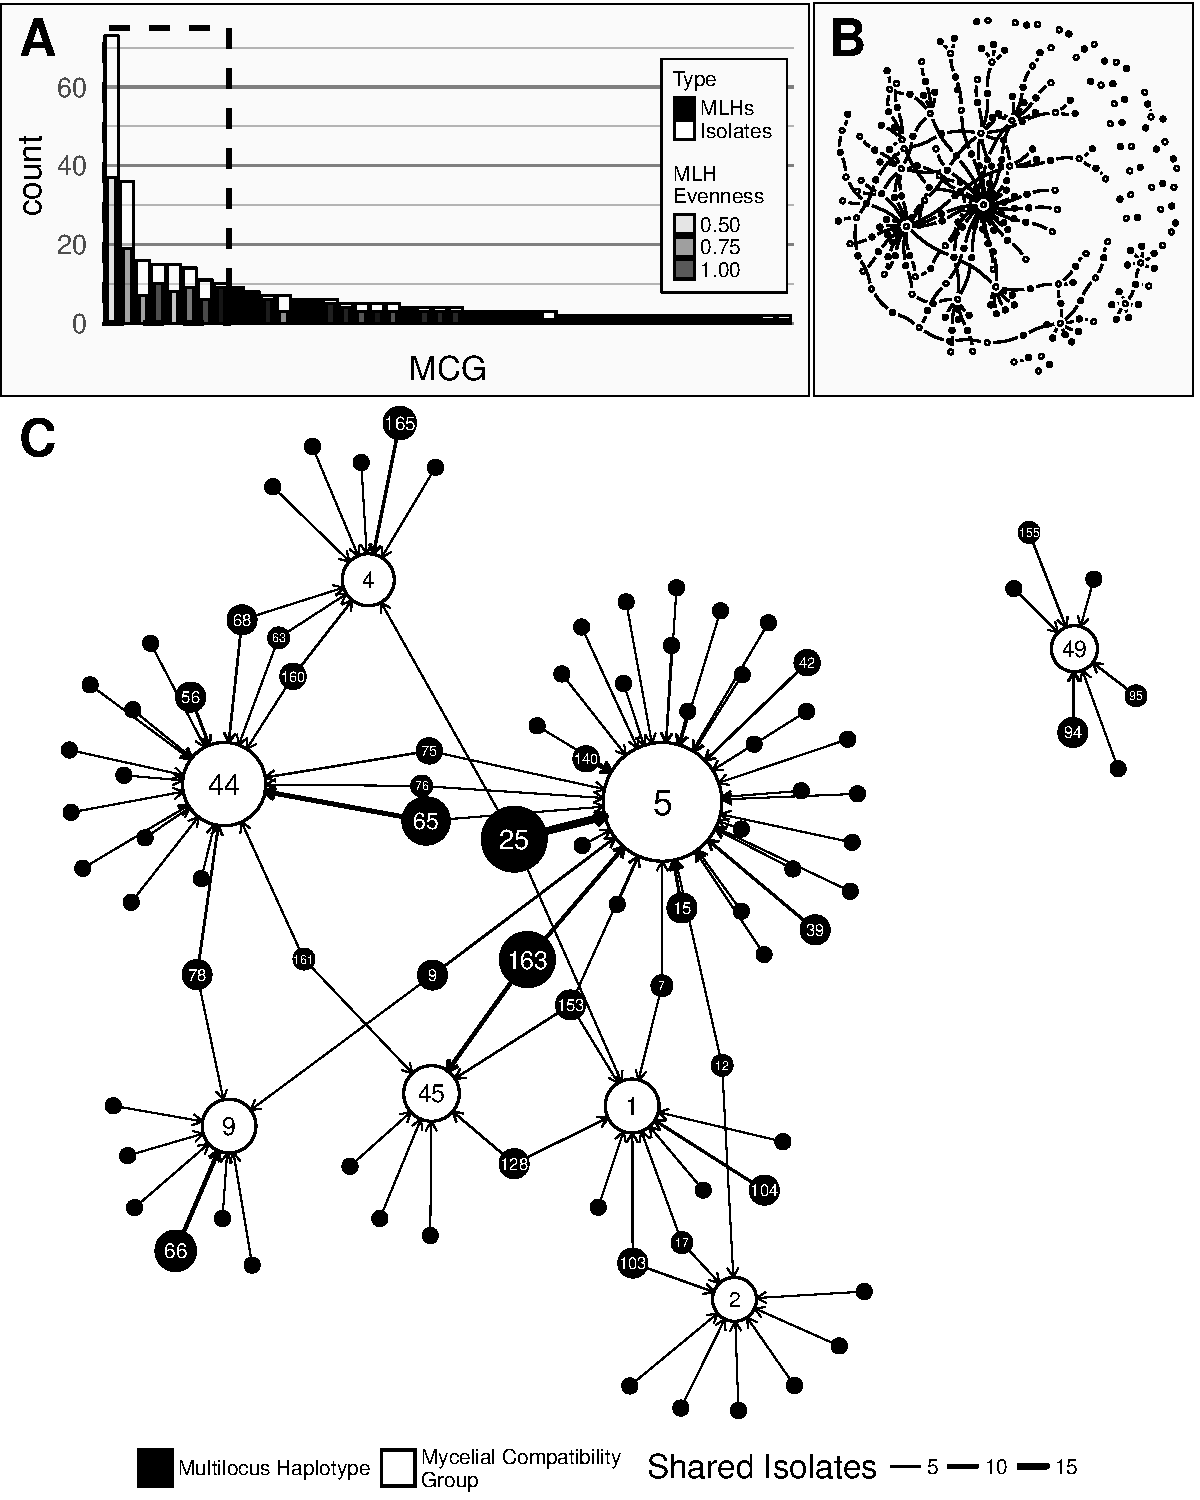
\includegraphics[width=1.00000\textwidth]{../../results/figures/publication/mcg-subgraph-with-context.pdf}
\caption{Associations between Mycelial Compatibility Groups and
Multilocus Haplotypes. \textbf{A)} Barplot of Mycelial Compatibility
Group (MCG) abundance in descending order. Singletons (46) were
truncated, leaving 41 MCGs. White bars represent sample counts and grey
bars represent counts of unique multilocus haplotypes (MLH). The
transparency of the bars represent the evenness of the distribution of
the MLHs within a given MCG. A dashed box surrounds the eight most
common MCGs representing \textgreater{}~51\% of the data. \textbf{B)}
Full graph-representation of the relationship between MCGs (open
circles) and MLHs (filled circles). Details in Fig. \ref{fullgraph}.
\textbf{C)} A subset of \textbf{B} representing the 8 most common MCGs
and their associated MLHs (dashed box in \textbf{A}). Filled nodes
(circles) represent MLHs and open nodes represent MCGs. Node area scaled
to the number of samples represented (range: 1--73). Numbers inside
nodes are the MLH/MCG label (if n \textgreater{} 1). Edges (arrows)
point from MLH to MCG where the weight (thickness) of the edge
represents the number of shared isolates (range: 1--19). Edges extending
from MLHs displayed to other MCGs are not shown.}\label{biggraph}
\end{figure}

\subsection*{Variable assessment}\label{variable-assessment}
\addcontentsline{toc}{subsection}{Variable assessment}

\subsubsection*{Variable contributions}\label{variable-contributions}
\addcontentsline{toc}{subsubsection}{Variable contributions}

\begin{figure}
\centering
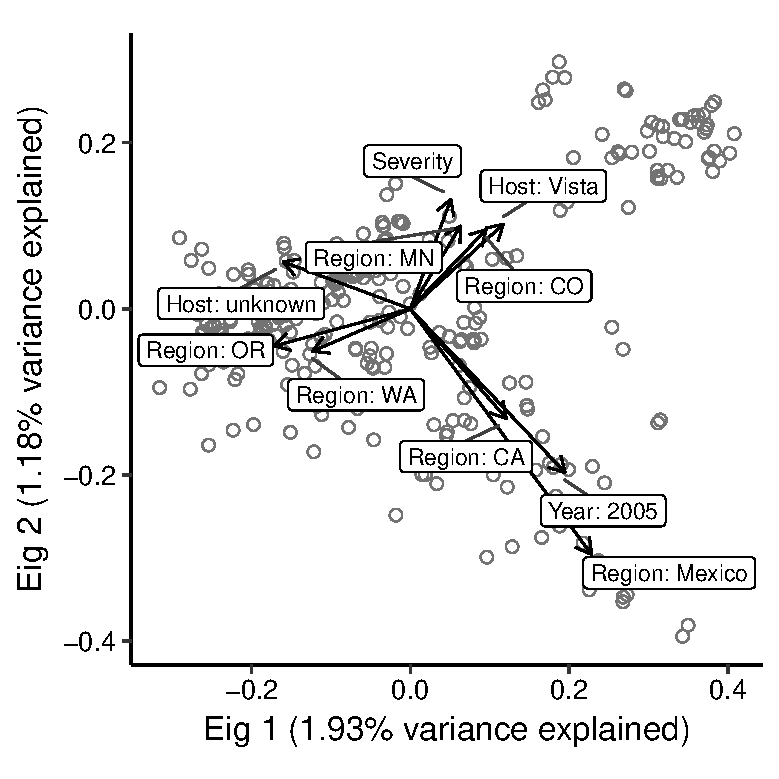
\includegraphics[width=0.61000\textwidth]{../../results/figures/publication/Figure7Z.pdf}
\caption{Biplot showing five most influential explanatory variables
(arrows) overlayed on the first two eigenvectors of distance based
redundancy analysis of \emph{Sclerotinia sclerotiorum} isolates. The
length of the arrows are directly proportional to the strength of the
correlation between explanatory and molecular variables. Open circles
represent the 318 clone-corrected haplotypes in ordination
space.}\label{rda-biplot}
\end{figure}

\begin{figure}
\centering
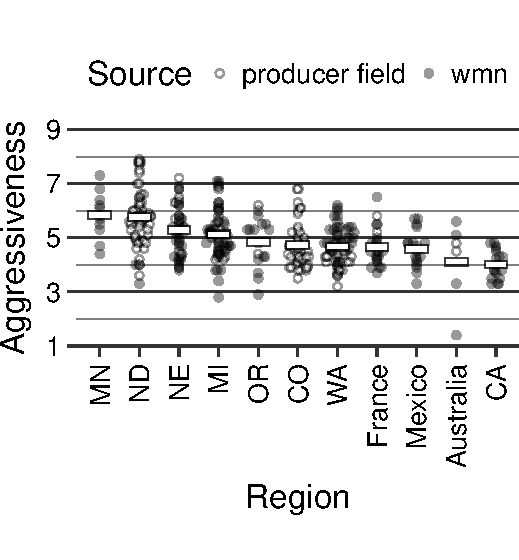
\includegraphics{../../results/figures/publication/aggressiveness.pdf}
\caption{Strip plot of aggressiveness by population arranged in
descending order of mean aggressiveness for all populations with N
\textgreater{} 5. White bars represent mean value. Circles represent
individual isolates where filled circles are isolates from white mold
screening nurseries (wmn) and open circles are isolates from producer
fields.}\label{aggressiveness-boxplot}
\end{figure}

The forward-backward selection process of the dbRDA models on
clone-corrected data revealed Year, Region, Host, and MCG to be the
optimal variables for the reduced model, accounting for 45\% of the
total variation. ANOVA showed that the reduced model was significant
with an adjusted R\textsuperscript{2} of 0.0675 (\emph{P} = 0.001).
Assessment of the marginal effects showed that all varibles
significantly explained genetic variation (\(P \leq 0.007\)). We found
that there was multicollinearity when MCG was combined with any other
variable, so repeated the analysis, dropping MCG from the list of
potential predictors. From these results, Year, Region, Host, and
Aggressiveness were found to be optimal, accounting for 17.6\% of the
total variation. ANOVA revealed significant effects with an adjusted
R\textsuperscript{2} of 0.0325 (\emph{P} = 0.001). While the marginal
effect assessment revealed that Year, Region, and Host significantly
explained variation at \emph{P} = 0.001, and Aggressiveness
significantly explained variation at \emph{P} = 0.039. Much of the
variation appeared to be driven by isolates from Mexico and 2005 (Fig.
\ref{rda-biplot}). Variance partitioning of the independent variables
without MCG indicated aggressiveness to be the least influential factor
with 0.1\% contributing to explaining the variation of molecular data,
whereas the combination of variables accounted for 3.3\%.

\subsubsection*{Aggressiveness}\label{aggressiveness-1}
\addcontentsline{toc}{subsubsection}{Aggressiveness}

Aggressiveness of the isolates ranged from 1.4 to 7.9 with a mean of
5.02 and median of 4.85. The group mean averages were 4.88, 5.13, and
5.19 for Region, MCG, and MLH, respectively. A strip plot showing the
distribution of severity across these three variables simultaneously can
be seen in Fig. \ref{mcg-mlh-region-aggressiveness}. Our assessment of
aggressiveness in association with Region showed a significant effect
(\emph{P} \textless{} 1.00e\textsuperscript{-4}), with means that ranged
from 5.8 (MN) to 4.0 (CA) (Fig. \ref{aggressiveness-boxplot}, Table
\ref{tab:region-aggressiveness}). MCGs also showed a significant effect
(\emph{P} \textless{} 0.001), with means that ranged from 6.0 (`MCG 44')
to 4.6 (`MCG 49'; Table \ref{tab:MCG-aggressiveness}). We additionally
found a significant effect for MLHs (\emph{P} \textless{} 0.001), with
means that ranged from 6.0 (`MLH 78') to 4.3 (`MLH 140') (Table
\ref{tab:MLG-aggressiveness}).

\subsubsection*{Correlation of mulitlocus haplotypes and mycelial
compatibility
groups}\label{correlation-of-mulitlocus-haplotypes-and-mycelial-compatibility-groups}
\addcontentsline{toc}{subsubsection}{Correlation of mulitlocus
haplotypes and mycelial compatibility groups}

In our analysis, we found 165 MLHs with 70 singletons and 87 MCGs with
43 singletons (Fig. \ref{biggraph}A,B) where the eight most abundant
MCGs represented \textgreater{} 51\% of the data over 11 Regions, and
all years except for 2012. Our network-based approach to correlating
MLHs with MCGs revealed a large and complex network (Fig.
\ref{biggraph}, Table \ref{tab:mlg-table}). Community analysis showed 51
communities, 15 of which consisted of a single MLH unconnected with any
other community indicating that just 9.09\% of the 165 MLHs are unable
to cross with any other MLH in this data set (Fig. \ref{fullgraph}). The
three communities with the most members contained eight of the 10 most
abundant MCGs. Comparing these communities with Bruvo's genetic distance
showed an average distance of 0.451 among communities and an average
distance of 0.437 within communities, which were not significantly
different. When we assessed the number of times two different MLHs that
are in the same MCG, considering these as potential heterothallic
pairings that could result in sexual recombination, we found an average
of 14.3 potential heterothallic parings per MLH. Representing just four
isolates, `MLH 75' had 57 neighbors that shared the same MCG (Fig.
\ref{biggraph}, \ref{fullgraph}). Overall, there was no clear pattern to
the association between MLH and MCGs.

\begin{longtable}[]{@{}llll@{}}
\caption{\label{tab:mlg-table} The five most abundant Multilocus Haplotypes
(MLH) with the probability of second encounter (\(P_{sex}\)), Mycelial
Compatibility Groups (MCG), and Regions with sample sizes in
parentheses.}\tabularnewline
\toprule
MLH & \(P_{sex}\) & MCG & Region\tabularnewline
\midrule
\endfirsthead
\toprule
MLH & \(P_{sex}\) & MCG & Region\tabularnewline
\midrule
\endhead
25 & 0.016824 & 5 & ND (15), CO (2), MI (2)\tabularnewline
& & 13 & ND (3)\tabularnewline
& & 60 & ND (2), WA (1)\tabularnewline
& & 1 & NE (1)\tabularnewline
& & 4 & MI (1)\tabularnewline
163 & 0.049932 & 45 & CO (5), ND (2), NE (1)\tabularnewline
& & 5 & MI (7)\tabularnewline
65 & 0.000071 & 44 & NE (10)\tabularnewline
& & 5 & MI (1)\tabularnewline
140 & 0.000155 & 8 & CO (5)\tabularnewline
& & 5 & MI (3)\tabularnewline
& & 20 & MI (2)\tabularnewline
66 & 0.000016 & 9 & NE (4), CO (2), MI (2)\tabularnewline
\bottomrule
\end{longtable}

\subsection*{Structure of shared multilocus
haplotypes}\label{structure-of-shared-multilocus-haplotypes}
\addcontentsline{toc}{subsection}{Structure of shared multilocus
haplotypes}

The most abundant MLH was represented by 27 isolates (Table
\ref{tab:mlg-table}) from five Regions (NE, MI, WA, CO, and ND). Within
Regions, haplotypes were relatively evenly distributed with moderate to
high diversity (Table \ref{tab:iatab}). Of the 165 MLHs, 76 (46\%) were
found in at least two Regions, except those found in WI (2), ID (1), and
Mexico (18) (Fig. \ref{community-graph}).

We had performed an analysis on a network where the connections
represented shared MLHs across populations, weighted by \(1 - P_{sex}\)
(Fig. \ref{community-graph}, Table \ref{tab:mlg-table}). Community
analysis of the MLHs shared between populations revealed 4 communities
with a modularity of 0.17: A coastal community (CA, OR, WA, and NY), a
Midwest community (CO, ND, NE, MI), and an international community
(Australia, France, MN). Although analysis with 16 loci resulted in the
removal of the NY node because it no longer shared a haplotype with OR,
the same overall community structure was present with a modularity of
0.2 (Fig. \ref{community-graph16}). Relative to the US, the
international community appears to be driven by MLH 4, which is shared
between all three populations and has a \(P_{sex}\) value of
2.87e\textsuperscript{-5}, in contrast to the abundant MLH 25, which has
a \(P_{sex}\) value of 0.0168.

\begin{figure}
\centering
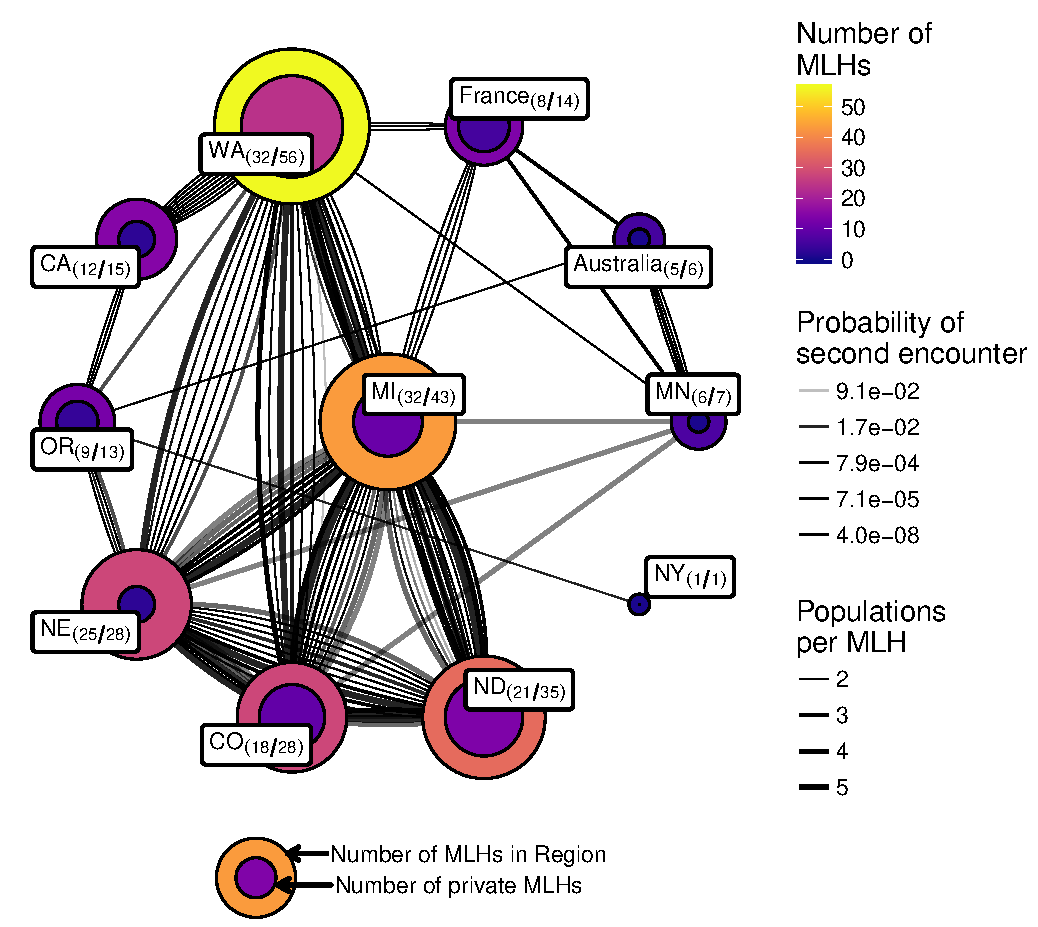
\includegraphics[width=0.61000\textwidth]{../../results/figures/publication/mlg-11.pdf}
\caption{Network of populations (nodes/circles) and their shared
multilocus haplotypes (MLH) (edges/lines) genotyped over 11 loci. Each
node is labeled with \textbf{name (number of MLHs shared/number of MLHs
total).} The shade and area of the nodes are proportional to the number
of unique MLHs within the node and the inner nodes are proportional to
the number of private MLHs to the region (bottom legend). Each edge
represents a single MLH where its thickness represents the number of
populations that share the MLH and the shade represents the value of
\(P_{sex}\), or the probability of encountering that MLH from two
independent meiotic events.}\label{community-graph}
\end{figure}

\subsection*{Population
differentiation}\label{population-differentiation-1}
\addcontentsline{toc}{subsection}{Population differentiation}

\subsubsection*{Analysis of molecular
variance}\label{analysis-of-molecular-variance}
\addcontentsline{toc}{subsubsection}{Analysis of molecular variance}

The AMOVA for clone-corrected samples over the hierarchy of Region,
Source, and Year showed significant variation between Regions and Years,
but no significant variation between wmn and producer fields (Table
\ref{tab:amova}). In contrast, when we compared the three cultivars,
Beryl, Bunsi, and G122, we found no significant differentiation (See
section on `Host Differentiation' in the
wmn-differentiation.md\footnote{Direct link:
  \url{https://github.com/everhartlab/sclerotinia-366/blob/master/results/wmn-differentiation.md\#host-differentiation}}
file in the supplemental files (Kamvar et al., 2017)).

\begin{longtable}[]{@{}clrllc@{}}
\caption{\label{tab:amova} Comparison of populations in the white mold
screening nurseries (wmn) and producer fields using an analysis of
molecular variance (AMOVA) on Bruvo's genetic distance showing no
apparent differentiation between wmn and other sources. The hierarchy
was constructed as Source/Region where source is defined as belonging to
a wmn or producer field. Bold \(\Phi\) values indicate significant
difference (\emph{P} \textless{} 0.05). S.S. = Sum of Squares, d.f. =
degrees of freedom.}\tabularnewline
\toprule
\begin{minipage}[b]{0.32\columnwidth}\centering\strut
Hierarchy\strut
\end{minipage} & \begin{minipage}[b]{0.06\columnwidth}\raggedright\strut
d.f.\strut
\end{minipage} & \begin{minipage}[b]{0.07\columnwidth}\raggedleft\strut
S.S.\strut
\end{minipage} & \begin{minipage}[b]{0.13\columnwidth}\raggedright\strut
\% variation\strut
\end{minipage} & \begin{minipage}[b]{0.19\columnwidth}\raggedright\strut
\(\Phi\) statistic\strut
\end{minipage} & \begin{minipage}[b]{0.07\columnwidth}\centering\strut
\emph{P}\strut
\end{minipage}\tabularnewline
\midrule
\endfirsthead
\toprule
\begin{minipage}[b]{0.32\columnwidth}\centering\strut
Hierarchy\strut
\end{minipage} & \begin{minipage}[b]{0.06\columnwidth}\raggedright\strut
d.f.\strut
\end{minipage} & \begin{minipage}[b]{0.07\columnwidth}\raggedleft\strut
S.S.\strut
\end{minipage} & \begin{minipage}[b]{0.13\columnwidth}\raggedright\strut
\% variation\strut
\end{minipage} & \begin{minipage}[b]{0.19\columnwidth}\raggedright\strut
\(\Phi\) statistic\strut
\end{minipage} & \begin{minipage}[b]{0.07\columnwidth}\centering\strut
\emph{P}\strut
\end{minipage}\tabularnewline
\midrule
\endhead
\begin{minipage}[t]{0.32\columnwidth}\centering\strut
Between Region\strut
\end{minipage} & \begin{minipage}[t]{0.06\columnwidth}\raggedright\strut
13\strut
\end{minipage} & \begin{minipage}[t]{0.07\columnwidth}\raggedleft\strut
10.19\strut
\end{minipage} & \begin{minipage}[t]{0.13\columnwidth}\raggedright\strut
8.45\strut
\end{minipage} & \begin{minipage}[t]{0.19\columnwidth}\raggedright\strut
\textbf{0.0845}\strut
\end{minipage} & \begin{minipage}[t]{0.07\columnwidth}\centering\strut
0.031\strut
\end{minipage}\tabularnewline
\begin{minipage}[t]{0.32\columnwidth}\centering\strut
Between Source within Region\strut
\end{minipage} & \begin{minipage}[t]{0.06\columnwidth}\raggedright\strut
8\strut
\end{minipage} & \begin{minipage}[t]{0.07\columnwidth}\raggedleft\strut
2.74\strut
\end{minipage} & \begin{minipage}[t]{0.13\columnwidth}\raggedright\strut
-2.29\strut
\end{minipage} & \begin{minipage}[t]{0.19\columnwidth}\raggedright\strut
-0.0250\strut
\end{minipage} & \begin{minipage}[t]{0.07\columnwidth}\centering\strut
0.497\strut
\end{minipage}\tabularnewline
\begin{minipage}[t]{0.32\columnwidth}\centering\strut
Between Year within Source\strut
\end{minipage} & \begin{minipage}[t]{0.06\columnwidth}\raggedright\strut
22\strut
\end{minipage} & \begin{minipage}[t]{0.07\columnwidth}\raggedleft\strut
9.37\strut
\end{minipage} & \begin{minipage}[t]{0.13\columnwidth}\raggedright\strut
16.28\strut
\end{minipage} & \begin{minipage}[t]{0.19\columnwidth}\raggedright\strut
\textbf{0.173}\strut
\end{minipage} & \begin{minipage}[t]{0.07\columnwidth}\centering\strut
0.001\strut
\end{minipage}\tabularnewline
\begin{minipage}[t]{0.32\columnwidth}\centering\strut
Within Year\strut
\end{minipage} & \begin{minipage}[t]{0.06\columnwidth}\raggedright\strut
274\strut
\end{minipage} & \begin{minipage}[t]{0.07\columnwidth}\raggedleft\strut
47.30\strut
\end{minipage} & \begin{minipage}[t]{0.13\columnwidth}\raggedright\strut
77.56\strut
\end{minipage} & \begin{minipage}[t]{0.19\columnwidth}\raggedright\strut
\textbf{0.224}\strut
\end{minipage} & \begin{minipage}[t]{0.07\columnwidth}\centering\strut
0.001\strut
\end{minipage}\tabularnewline
\bottomrule
\end{longtable}

\newpage

\subsubsection*{Discriminant analysis of principal
components}\label{discriminant-analysis-of-principal-components}
\addcontentsline{toc}{subsubsection}{Discriminant analysis of principal
components}

DAPC was performed by grouping Region with the first 21 principal
components, representing 88.1\% of the total variance. The first
discriminant axis (representing 63.9\% of the discriminatory power)
separated the centroid for the Mexico isolates from the rest of the
data, indicating strong differentiation (Fig. \ref{DAPC}b). The second
discriminant axis, representing 10.8\% of the discriminatory power,
separated the centroid for the CA isolates. The mean population
assignment probabilities for all populations with n \textgreater{} 10
showed that only isolates from Mexico, CA, and France had \textgreater{}
50\% probabilities of being reassigned to their source populations (Fig.
\ref{DAPC}a).

DAPC grouping by cultivar used the first 20 principal components,
representing 89\% of the total variance. The first two discriminant axes
(representing 100\% of the discriminatory power) failed to separate any
of the cultivars where the mean posterior assignment probabilities were
34\% (G122), 35.9\% (Beryl), and 30.1\% (Bunsi). DAPC grouping by Region
and Year used the first 15 principal components, representing 80.3\% of
the total variance. The North Central USA populations (NE, MI, CO, ND)
did not appear to have any variation across time in contrast to WA,
which showed a shift in population structure in the last year of
sampling, 2008 (Fig. \ref{DAPC-RY}). Further analysis of this population
revealed that all 12 isolates in WA circa 2008 originated in a wmn; nine
haplotypes were shared with CA, and three were shared with France (Fig.
\ref{community-graph}, \ref{community-graph16}).

\begin{figure}
\centering
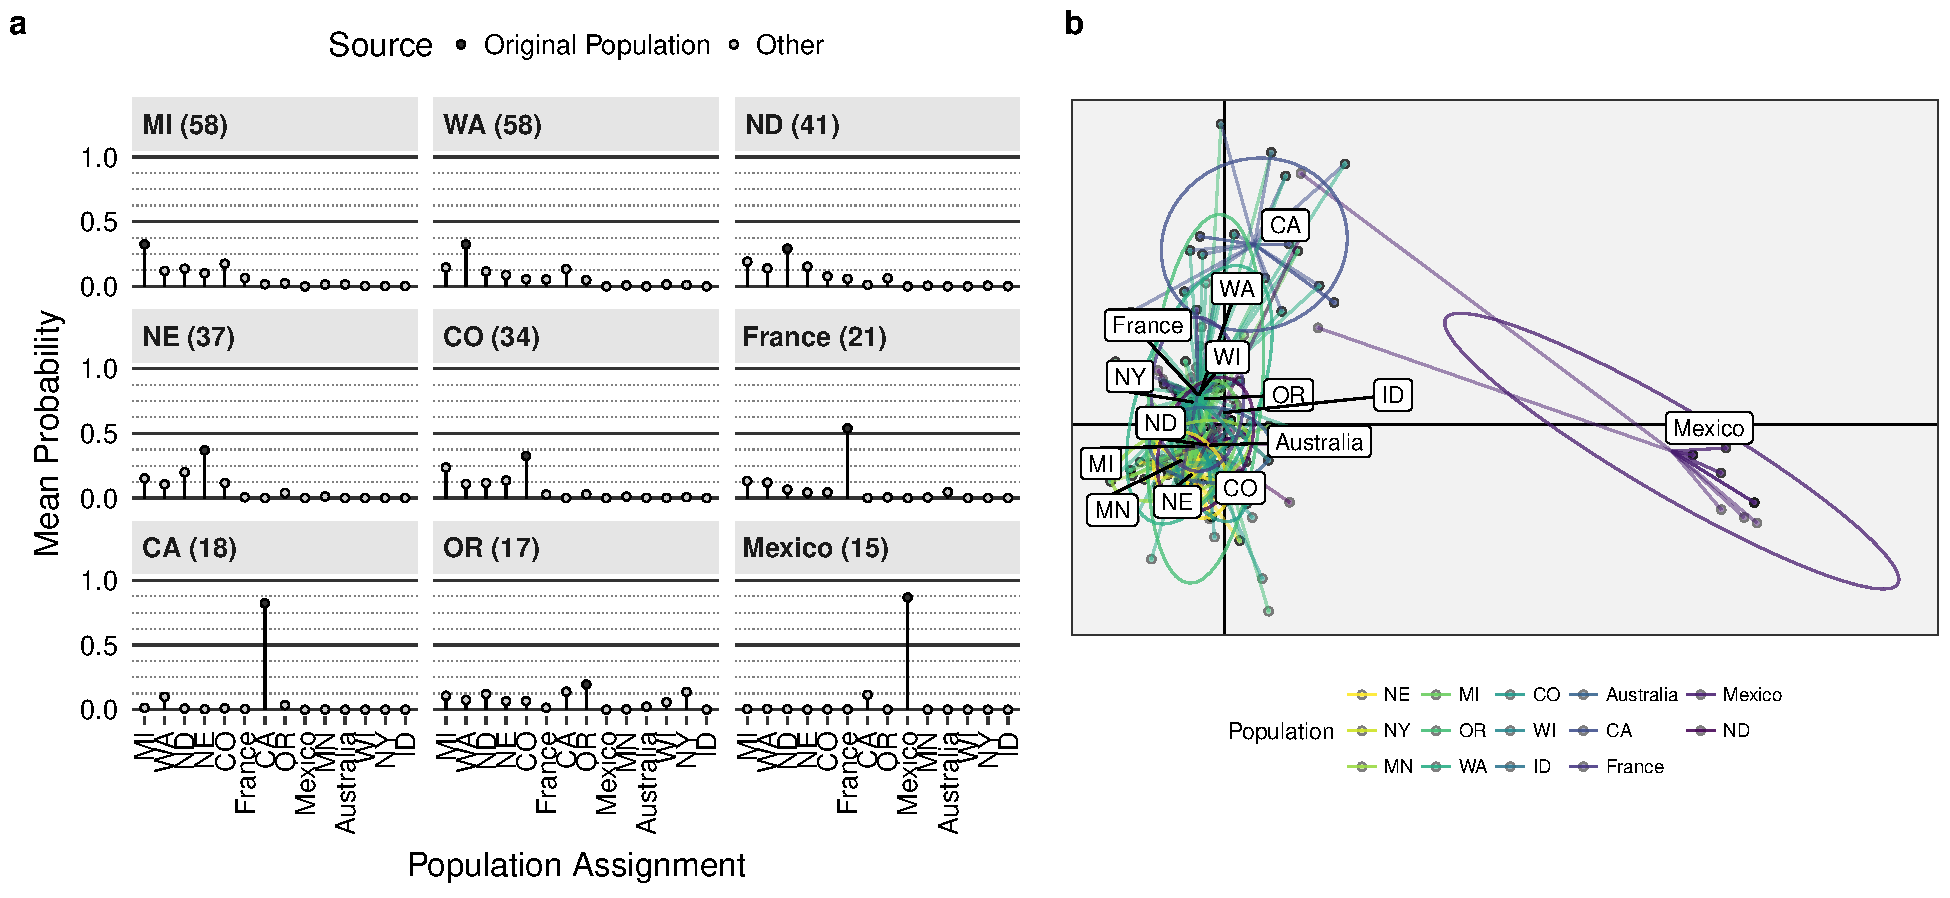
\includegraphics[width=1.00000\textwidth]{../../results/figures/publication/DAPC.pdf}
\caption{Discriminant Analysis of Principal Components (DAPC) on regions
showing that Mexico is differentiated from other populations.
\textbf{A)} Scatter plot of first two components from DAPC. Points
represent observed individuals connected to the population centroids
with ellipses representing a 66\% confidence interval for a normal
distribution. The center of each component is represented as black grid
lines. \textbf{B)} Mean population assignment probability from the DAPC
for all populations with N \textgreater{} 10 (facets). Populations
represented along the horizontal axis and probability of assignment on
the vertical. Numbers next to source populations indicate population
size. All values sum to one.}\label{DAPC}
\end{figure}

\begin{figure}
\centering
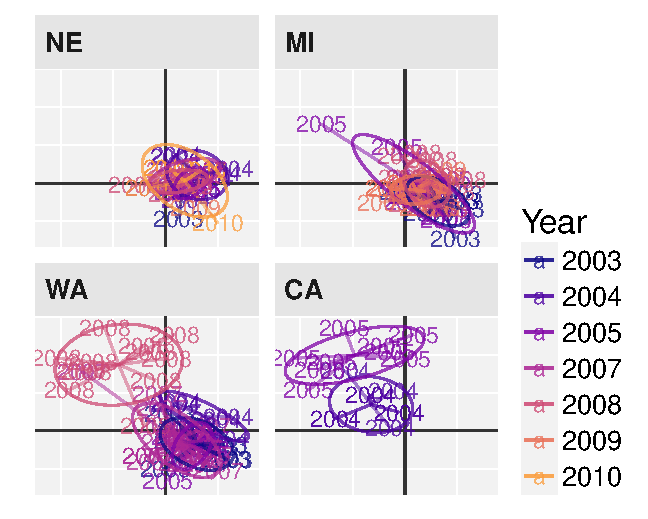
\includegraphics[width=0.61000\textwidth]{../../results/figures/publication/dapc_region_year_micanewa.pdf}
\caption{Scatter plot of Discriminant Analysis of Principal Components
(DAPC) on Regions and Years showing non-differentiated temporal
variation NE and MI and temporal variation in WA and CA. Points (text
labels) represent observed individuals connected to the population
centroids with ellipses representing a 66\% confidence interval for a
normal distribution. The center of each component is represented as
black grid lines. A more detailed view is shown in Fig.
\ref{DAPC-RY-FULL}.}\label{DAPC-RY}
\end{figure}

\section*{Discussion}\label{discussion}
\addcontentsline{toc}{section}{Discussion}

In this study, we characterized the diversity of \emph{Sclerotinia
sclerotiorum} from dry bean fields across the United States. Our results
suggest that, broadly, populations from white mold screening nurseries
reflect the populations of the surrounding regions, indicating that
resistance screening may be successful within regions. We found
significant population differentiation by geographic region and year,
mainly differentiated into three broad North American groups based on
shared haplotypes and posterior groupings, a Coastal Region, Midwestern
Region, and Mexico. To date, with 366 isolates, this is the largest
single population genetic study of \emph{S. sclerotiorum} assessing
population structure within managed and unmanaged agricultural
environments. These findings indicate that the white mold screening
nurseries can be effective at screening for potential resistant lines
within growing regions.

We found that the best predictors of genetic structure are Region and
Year, supporting the hypothesis that \emph{S. sclerotiorum} populations
are spatially structured (Carbone \& Kohn, 2001). Borrowing a technique
often used in the ecological literature, we used dbRDA to elucidate the
effect of all variables (MCG, Region, Source, Year, Host, and
Aggressiveness) (Legendre \& Anderson, 1999). From the initial results,
it appeared that the most important factors for predicting genetic
structure were MCG, region, and year. When we inspected the biplot of
the initial results, we saw that the most important predictors were `MCG
44', `MCG 5', and `MCG 9'. We believe that this was driven by the fact
that these particular MCGs have uneven MLH distributions, meaning that
they are heavily associated with one particular MLH (Fig.
\ref{biggraph}). We note these results with caution because of the
apparent multicolinearity between MCG and Region, which is a violation
of the analysis (Legendre \& Anderson, 1999). While the results
indicated that Mexico and the year 2005 were the two most important
variables, it's worth noting that all Mexico isolates were collected in
2005 (Fig. \ref{rda-biplot}). The results also show that the Vista
cultivar explains some of the variance, but this represents six isolates
in MI, and thus we cannot draw broad conclusions from this axis.
Aggressiveness and source field had little to no effect on prediction of
genetic diversity. These results are in agreement with studies that
examined differentiation based on Host (Aldrich-Wolfe et al., 2015) and
Aggressiveness (Atallah et al., 2004; Attanayake et al., 2012, 2013)
reporting little or no correlation of genetic diversity to these
variables. This indicates that a) breeders should keep in mind regional
differences when assessing resistance and b) it is possible that we have
not yet measured biologically relevant variables that can predict
genetic differentiation, which could include variables such as soil
community composition.

While aggressiveness was not shown to predict genetic structure, it is
an important factor in breeding efforts, and we observed significant
differences in aggressiveness based on Region (Fig.
\ref{aggressiveness-boxplot}, Table \ref{tab:region-aggressiveness}).
These results show a similar pattern to what was found previously in
Otto-Hanson et al. (2011) with the exception of North Dakota, which
increased in mean aggressiveness from 5 to 5.77. This increase was due
in part to new data from producer field isolates collected after the
previous study. These straw tests were performed by a different person
for these later isolates, which could suggest a more lenient or strict
scoring system. However, when we examined the within-region differences,
we found no significant effect by individual. Many of the ND isolates
fell within the 6--7 range, which denotes a physical boundary (disease
symptoms around the second node) between intermediate and susceptible
(Otto-Hanson et al., 2011). Thus, we observed a shift in aggressiveness
without a significant shift in genotypic structure, which may indicate
that aggressiveness may be controlled by environmental factors as
opposed to genetic profile.

The primary interest of this study was to assess if isolates sampled
from white mold screening nurseries represent isolates from producer
fields within the region (Steadman et al., 2003; Otto-Hanson et al.,
2011). According to our AMOVA results, we have evidence for
differentiation at the Region and Year, but little to no differentiation
between wmn isolates and production field isolates (Table
\ref{tab:amova}). This lack of differentiation, however, may reflect the
breeder practice of inoculating screening plots with sclerotia collected
from sources within the region. When we analyze the AMOVA results in
light of the DAPC results (Fig. \ref{DAPC}), it becomes clear that the
regional patterns of differentiation are largely driven by isolates from
Mexico and CA. Isolates from these Regions had a higher posterior
probability (\textgreater{} 0.75) of being reassigned to their own
populations than any other (Fig. \ref{DAPC}A). All other populations in
comparison (except France) has reassignment probabilities of \textless{}
0.5, which is reflected in the failure of the first two discriminant
functions to separate these populations (Fig. \ref{DAPC}B).

Despite the evidence that Mexico and CA contributed to much of the
population differentiation, Regions like WA still had a large amount of
internal variation. The two distinct clusters for the WA Region showed
that the 2008 population appeared differentiated and, under further
investigation, we found that all the haplotypes from this year were
shared between CA and France (Fig. \ref{community-graph}, \ref{DAPC-RY},
\ref{DAPC-RY-FULL}). All of the isolates from WA in 2003--2005, and 2008
came from the same wmn; within the wmn, those in 2003--2005 came a
Northeastern field location cropped with dry bean since 2002, and those
in 2008 from a Southeastern field that was previously cropped with
brassica, sundgrass, peas, beans, and potatoes (Miklas, Phil Pers.
comm.). Both of these fields were inoculated with sclerotia in 2002, the
Northeastern field with sclerotia provided by a commercial bean producer
and the Southeastern field with sclerotia from peas (although this was
thought to be unsuccessful). Despite this information, it is still
unclear what has contributed to the differentiation of the 2008
population from WA or why it shares haplotypes with CA and France. When
we assessed agressiveness between the two fields across years with an
ANOVA model, we found that there was a slight effect based on field (P =
0.0127). While the evidence may suggest host as being a factor, previous
studies have shown no significant differentiation across host species
(Aldrich-Wolfe et al., 2015). It was of interest to compare our data
with that of Aldrich-Wolfe et al. (2015), but we found that, due to
differences in data generation, we were unable to confidently perform a
comparison (See supplemental file compare-aldrich-wolfe.md\footnote{Direct
  link:
  \url{https://github.com/everhartlab/sclerotinia-366/blob/master/results/compare-aldrich-wolfe.md}}
(Kamvar et al., 2017)).

With the exception of the WA Region, populations that were sampled
across several years appeared to be relatively stable over time with
overlapping distributions in the DAPC (i.e.~NE and MI, Fig.
\ref{DAPC-RY}). DAPC is based on the principal components of allele
counts (Jombart et al., 2010). Unlike Bruvo's distance, this does not
take into account the magnitude of the difference between alleles, which
could inflate the distance measure in the presence of private alleles
(Bruvo et al., 2004). While we found no evidence of private alleles in
the Mexico and CA isolates, we did find that the alleles driving the
first axis in Fig. \ref{DAPC}A (alleles 174, 256, and 372 in loci 7-2,
8-3, and 9-2, respectively) were overrepresented in Mexico (where
\textgreater{}75\% of the alleles came from the region). However, all
three of these alleles, i) conform to the expected stepwise mutation
model (Bruvo et al., 2004) and ii) are at or near the extremes of the
total range (except for allele 372 at locus 9-2). Moreover, the fact
that we find three alleles at three independent loci segregating the
Mexican genotypes suggests that the pattern separating these populations
from the others was not an artifact. We believe that the differences in
populations observed from Mexico may be due to differences in climate
that allow greater diversification via sexual outcrossing.

Many of the isolates in our study were from temperate climates and the
only isolates representing a sub-tropical climate were from Mexico. It
has been proposed within the \emph{S. sclerotiorum} literature that
isolates from sub-tropical and tropical climates are differentiated or
more variable than populations from temperate climates (Carbone \& Kohn,
2001; Attanayake et al., 2013; Lehner \& Mizubuti, 2017). This has been
attributed to the notion that the fungus has the chance to undergo more
reproductive cycles in the warmer climate (Carbone \& Kohn, 2001;
Attanayake et al., 2013). The strongest evidence to date supporting this
hypothesis is from Attanayake et al. (2013), showing that populations in
sub-tropical regions of China have been found to be more variable,
sexually reproducing, and unrelated to populations in temperate regions
of the USA. This result however, may be driven more by geography and
agricultural practice as opposed to climate.

The results from our shared haplotype analysis showed several
populations with at least one haplotype between them, except for Mexico
and two states that had fewer than three samples each (Fig.
\ref{community-graph}). Our network-based approach by treating the
haplotypes as edges and weighting each edge with the inverse of
\(P_{sex}\) treated the edges as springs connecting the populations with
the strength proportional to the probability of obtaining the same
haplotype as a clone. This allowed us to use a graph walking algorithm
to see how close the populations were, simply based off of the
proportion of clones they shared. The most abundant haplotype was shared
across four populations, but its high value of \(P_{sex}\) meant that it
did not contribute significantly to the overall structure. The graph
walking algorithm was able to divide the network into three groups, but
had a modularity of 0.17, which indicates that the groups are only
weakly differentiated.

The widespread nature of multilocus haplotypes in both wmn and
production fields with relatively small values of \(P_{sex}\) may
indicate the spread of inoculum between regions. While seedborne
transmission is thought to be of insignificant epidemiological
importance (Strausbaugh \& Forster, 2003), it has since been shown that
\emph{S. sclerotiorum} infections can be transmitted through seed
(Botelho et al., 2013). Thus, we hypothesize that shared haplotypes
between populations may arise due to transmission events of seed or
sclerotia. This could explain the fact that we see shared haplotypes
with low \(P_{sex}\) values shared between Australia, France, and the
United States. While we speculate that these transmission events are
rare due to the genetic structuring by Region, these results suggest
that seedborne infections may indeed reflect a source of inoculum. This
may, in turn increase the risk of introducing new sources of genetic
variation through potential outcrossing events.

When we tested for sexual reproduction, we were unable to find evidence
for it in any region except for Australia and CA. While the Australia
population had a non-significant value of \(\bar{r}_d\)---which would
suggest that we cannot reject the null hypothesis of random mating---the
sample size was insufficient from which to draw conclusions (Milgroom,
1996; Agapow \& Burt, 2001). The low value of \(\bar{r}_d\) in the CA
population may represent sexual reproduction, but we can see in Fig.
\ref{DAPC-RY} that there is differentiation by year. Thus, this could
also be an artifact of sampling two different populations, which is
known to reduce the value of \(\bar{r}_d\) (Prugnolle \& de Meeûs,
2010).

The previous study of the white mold screening nursery populations used
MCGs to assess genotypic diversity (Otto-Hanson et al., 2011).
Historically, MCGs have been used as a proxy for clonal lineages, and
thus, of interest in this study was testing the association between
multilocus haplotypes (MLHs) and mycelial compatibility groups (MCGs)
(Kohn et al., 1990; Leslie, 1993; Kohn, 1995; Carbone et al., 1999;
Schafer \& Kohn, 2006; Otto-Hanson et al., 2011). Our results, however,
do not support this assumption. It can be seen in Fig. \ref{biggraph}A
that the most abundant MCG contains several MLHs, but the diversity of
those MLHs are low as indicated by the evenness (transparency), which
indicates that there is one dominant MLH (`MLH 25'). What is not shown
in Fig. \ref{biggraph}A is the MLHs that are shared between MCGs. This
is illustrated in both Table \ref{tab:mlg-table} and Fig.
\ref{biggraph}B,C. It could be argued, however that `MLH 25', with its
high value of \(P_{sex}\) represents different true MLHs across the five
MCGs it occupies, but this does not account for the overall structure of
Fig. \ref{fullgraph} where, for example, `MLH 75' (\(P_{sex}\) =
1.81e\textsuperscript{-4}) is compatible with 57 other haplotypes
through three MCG when the population structure of \emph{S.
sclerotiorum} is known to be clonal.

Over the past few years, researchers have noticed inconsistencies among
the relationship between MCGs and MLHs (Carbone et al., 1999; Attanayake
et al., 2012; Aldrich-Wolfe et al., 2015; Lehner et al., 2015). Either
several MCGs belong to one MLH, which could be explained by insufficient
sampling of loci; several MLHs belong to one MCG, which could be
explained by clonal expansion; or a mixture of both. Some studies have
shown a correlation between MCG and MLH (Carbone et al., 1999;
Aldrich-Wolfe et al., 2015; Lehner et al., 2015), whereas other studies
have shown no apparent correlation, even on small spatial scales
(Atallah et al., 2004; Attanayake et al., 2012, 2013).

One long-held assumption was that MCGs (as determined via barrage
reaction) represent vegetative compatibility groups (VCGs) (Kohn et al.,
1990; Schafer \& Kohn, 2006; Lehner et al., 2015), which are known to
have a genetic component (Saupe, 2000; Hall et al., 2010; Strom \&
Bushley, 2016). While our protocol for assessing MCGs utilized Diana
Sermons Medium (Cubeta et al., 2001) as compared to Patterson's Medium
or Potato Dextrose Agar (Schafer \& Kohn, 2006) for the MCG reactions,
the patterns we observe are not dissimilar from what have previously
been reported in the literature. It has been demonstrated in several
Ascomycetes---including \emph{Neurospora crassa} (Micali \& Smith,
2003), \emph{Sclerotinia homoeocarpa} (Jo et al., 2008),
\emph{Verticillium dahliae} (Papaioannou \& Typas, 2014), and \emph{S.
sclerotiorum} (Ford et al., 1995)---that barrage reactions are
independent from stable anastomosis. Thus, the inconsistencies in this
study and other studies indicate that researchers studying \emph{S.
sclerotiorum} should not rely on MCG data derived from barrage reactions
as an indicator for genetic diversity.

\subsection*{Limitations}\label{limitations}
\addcontentsline{toc}{subsection}{Limitations}

One of the main limitations of this study is the focus on \emph{P.
vulgaris} as a host. It has been shown that \emph{S. sclerotiorum} in
the midwestern United States does not have a particular preference for
host (Aldrich-Wolfe et al., 2015). If the distribution of \emph{S.
sclerotiorum} is even across agricultural hosts in the USA, then our
sample may yet be representative of the genetic pool present in other
crops and weedy species. Additionally, while we found no signficant
association between genotype and aggressiveness, it is important to note
that the straw test is only one measure of aggressiveness. Additional
phenotypes for aggressiveness should be evaluated for future studies.

Another limitation was the microsatellite markers used for this
particular study (Sirjusingh \& Kohn, 2001). The haplotype accumulation
curve showed no indication of a plateau, indicating that if we had
sampled more loci, we would have resolved more multilocus haplotypes.
While 16 loci showed us similar results and began to show a plateau for
the haplotype accumulation curve, we were unable to use these results
due to our uncertainty in the allele calls for these five extra loci.
With the availability of an optically-mapped genome (Derbyshire et al.,
2017), future studies describing the genetic diversity of \emph{S.
sclerotiorum} should employ techniques such as Genotyping-By-Sequencing
(Davey et al., 2011), Sequence Capture (Grover et al., 2012), or Whole
Genome Sequencing.

\subsection*{Conclusions}\label{conclusions}
\addcontentsline{toc}{subsection}{Conclusions}

This study represents the largest genetic analysis of \emph{S.
sclerotiorum} from the USA to date, giving us a unique insight to
continent-wide population structure and relationships between phenotypic
and genotypic variables. Populations in wmn appear to show no
significant differentiation when compared to their production field
counterparts, suggesting that the wmn populations of \emph{S.
sclerotiorum} may be considered representative of the surrounding
regions. While we found no direct relationship between haplotype and
severity, it is evident that there is a gradient of severity by region,
further supporting the need for screening in multiple locations. Based
on our analysis of the relationships between MCG and MLH, we found no
clear evidence that the two are directly related, suggesting that MCG
does not necessarily represent vegetative compatibility groups and thus
should not be used as a proxy for identifying clones.

\subsection*{Data Availability}\label{data-availability}
\addcontentsline{toc}{subsection}{Data Availability}

All scripts, data, and resources used to generate the results presented
in this publication (including Supplementary Information) are fully
reproducible and available at The Open Science Framework
\url{https://osf.io/ejb5y} (Kamvar et al., 2017).

\subsection*{Acknowledgements}\label{acknowledgements}
\addcontentsline{toc}{subsection}{Acknowledgements}

The authors would like to thank Rebecca Higgins for technical support in
generating the data for the MCG assessment, aggressiveness ratings, and
genotyping; and for providing valuable insights into the historical
context of the data collection and curation.

We would also like to thank Denita Hadziabdic and two other anonymous
reviewers for their valuable comments and insights that improved the
quality of the manuscript.

\newpage

\section*{Supplementary Information}\label{supplementary-information}
\addcontentsline{toc}{section}{Supplementary Information}

\setcounter{table}{0} \renewcommand{\thetable}{S\arabic{table}}
\setcounter{figure}{0} \renewcommand{\thefigure}{S\arabic{figure}}

\begin{longtable}[]{@{}lllrlr@{}}
\caption{\label{tab:isolate-table} Description of \emph{Sclerotinia
sclerotiorum} isolates used in this study. N = Number of Isolates. Key
abbreviations: wmn = white mold screening nursery, producer = producer
field, unk = unknown cultivar.}\tabularnewline
\toprule
\begin{minipage}[b]{0.11\columnwidth}\raggedright\strut
Country\strut
\end{minipage} & \begin{minipage}[b]{0.08\columnwidth}\raggedright\strut
State\strut
\end{minipage} & \begin{minipage}[b]{0.12\columnwidth}\raggedright\strut
Field Code\strut
\end{minipage} & \begin{minipage}[b]{0.19\columnwidth}\raggedleft\strut
Year\strut
\end{minipage} & \begin{minipage}[b]{0.29\columnwidth}\raggedright\strut
Host\strut
\end{minipage} & \begin{minipage}[b]{0.04\columnwidth}\raggedleft\strut
N\strut
\end{minipage}\tabularnewline
\midrule
\endfirsthead
\toprule
\begin{minipage}[b]{0.11\columnwidth}\raggedright\strut
Country\strut
\end{minipage} & \begin{minipage}[b]{0.08\columnwidth}\raggedright\strut
State\strut
\end{minipage} & \begin{minipage}[b]{0.12\columnwidth}\raggedright\strut
Field Code\strut
\end{minipage} & \begin{minipage}[b]{0.19\columnwidth}\raggedleft\strut
Year\strut
\end{minipage} & \begin{minipage}[b]{0.29\columnwidth}\raggedright\strut
Host\strut
\end{minipage} & \begin{minipage}[b]{0.04\columnwidth}\raggedleft\strut
N\strut
\end{minipage}\tabularnewline
\midrule
\endhead
\begin{minipage}[t]{0.11\columnwidth}\raggedright\strut
USA\strut
\end{minipage} & \begin{minipage}[t]{0.08\columnwidth}\raggedright\strut
CA\strut
\end{minipage} & \begin{minipage}[t]{0.12\columnwidth}\raggedright\strut
wmn\strut
\end{minipage} & \begin{minipage}[t]{0.19\columnwidth}\raggedleft\strut
2004, 2005\strut
\end{minipage} & \begin{minipage}[t]{0.29\columnwidth}\raggedright\strut
Beryl, Bunsi, G122\strut
\end{minipage} & \begin{minipage}[t]{0.04\columnwidth}\raggedleft\strut
18\strut
\end{minipage}\tabularnewline
\begin{minipage}[t]{0.11\columnwidth}\raggedright\strut
USA\strut
\end{minipage} & \begin{minipage}[t]{0.08\columnwidth}\raggedright\strut
CO\strut
\end{minipage} & \begin{minipage}[t]{0.12\columnwidth}\raggedright\strut
producer\strut
\end{minipage} & \begin{minipage}[t]{0.19\columnwidth}\raggedleft\strut
2007, 2010\strut
\end{minipage} & \begin{minipage}[t]{0.29\columnwidth}\raggedright\strut
Pinto, Yellow\strut
\end{minipage} & \begin{minipage}[t]{0.04\columnwidth}\raggedleft\strut
41\strut
\end{minipage}\tabularnewline
\begin{minipage}[t]{0.11\columnwidth}\raggedright\strut
\strut
\end{minipage} & \begin{minipage}[t]{0.08\columnwidth}\raggedright\strut
\strut
\end{minipage} & \begin{minipage}[t]{0.12\columnwidth}\raggedright\strut
wmn\strut
\end{minipage} & \begin{minipage}[t]{0.19\columnwidth}\raggedleft\strut
2003\strut
\end{minipage} & \begin{minipage}[t]{0.29\columnwidth}\raggedright\strut
GH\strut
\end{minipage} & \begin{minipage}[t]{0.04\columnwidth}\raggedleft\strut
1\strut
\end{minipage}\tabularnewline
\begin{minipage}[t]{0.11\columnwidth}\raggedright\strut
USA\strut
\end{minipage} & \begin{minipage}[t]{0.08\columnwidth}\raggedright\strut
ID\strut
\end{minipage} & \begin{minipage}[t]{0.12\columnwidth}\raggedright\strut
producer\strut
\end{minipage} & \begin{minipage}[t]{0.19\columnwidth}\raggedleft\strut
2003\strut
\end{minipage} & \begin{minipage}[t]{0.29\columnwidth}\raggedright\strut
GH\strut
\end{minipage} & \begin{minipage}[t]{0.04\columnwidth}\raggedleft\strut
1\strut
\end{minipage}\tabularnewline
\begin{minipage}[t]{0.11\columnwidth}\raggedright\strut
USA\strut
\end{minipage} & \begin{minipage}[t]{0.08\columnwidth}\raggedright\strut
MI\strut
\end{minipage} & \begin{minipage}[t]{0.12\columnwidth}\raggedright\strut
wmn\strut
\end{minipage} & \begin{minipage}[t]{0.19\columnwidth}\raggedleft\strut
2003, 2004, 2005, 2008, 2009\strut
\end{minipage} & \begin{minipage}[t]{0.29\columnwidth}\raggedright\strut
11A, 37, 38, B07104, Beryl, Bunsi, Cornell, G122, Orion, PO7863,
WM31\strut
\end{minipage} & \begin{minipage}[t]{0.04\columnwidth}\raggedleft\strut
43\strut
\end{minipage}\tabularnewline
\begin{minipage}[t]{0.11\columnwidth}\raggedright\strut
\strut
\end{minipage} & \begin{minipage}[t]{0.08\columnwidth}\raggedright\strut
\strut
\end{minipage} & \begin{minipage}[t]{0.12\columnwidth}\raggedright\strut
producer\strut
\end{minipage} & \begin{minipage}[t]{0.19\columnwidth}\raggedleft\strut
2003, 2008, 2009\strut
\end{minipage} & \begin{minipage}[t]{0.29\columnwidth}\raggedright\strut
BL, Black, Fuji, GH, Merlot, SR06233, unk, Vista, Zorro\strut
\end{minipage} & \begin{minipage}[t]{0.04\columnwidth}\raggedleft\strut
19\strut
\end{minipage}\tabularnewline
\begin{minipage}[t]{0.11\columnwidth}\raggedright\strut
USA\strut
\end{minipage} & \begin{minipage}[t]{0.08\columnwidth}\raggedright\strut
MN\strut
\end{minipage} & \begin{minipage}[t]{0.12\columnwidth}\raggedright\strut
wmn\strut
\end{minipage} & \begin{minipage}[t]{0.19\columnwidth}\raggedleft\strut
2003, 2004\strut
\end{minipage} & \begin{minipage}[t]{0.29\columnwidth}\raggedright\strut
Beryl, Bunsi, G122\strut
\end{minipage} & \begin{minipage}[t]{0.04\columnwidth}\raggedleft\strut
11\strut
\end{minipage}\tabularnewline
\begin{minipage}[t]{0.11\columnwidth}\raggedright\strut
USA\strut
\end{minipage} & \begin{minipage}[t]{0.08\columnwidth}\raggedright\strut
ND\strut
\end{minipage} & \begin{minipage}[t]{0.12\columnwidth}\raggedright\strut
producer\strut
\end{minipage} & \begin{minipage}[t]{0.19\columnwidth}\raggedleft\strut
2007, 2010\strut
\end{minipage} & \begin{minipage}[t]{0.29\columnwidth}\raggedright\strut
unk\strut
\end{minipage} & \begin{minipage}[t]{0.04\columnwidth}\raggedleft\strut
53\strut
\end{minipage}\tabularnewline
\begin{minipage}[t]{0.11\columnwidth}\raggedright\strut
\strut
\end{minipage} & \begin{minipage}[t]{0.08\columnwidth}\raggedright\strut
\strut
\end{minipage} & \begin{minipage}[t]{0.12\columnwidth}\raggedright\strut
wmn\strut
\end{minipage} & \begin{minipage}[t]{0.19\columnwidth}\raggedleft\strut
2005\strut
\end{minipage} & \begin{minipage}[t]{0.29\columnwidth}\raggedright\strut
Beryl, Bunsi, G122\strut
\end{minipage} & \begin{minipage}[t]{0.04\columnwidth}\raggedleft\strut
7\strut
\end{minipage}\tabularnewline
\begin{minipage}[t]{0.11\columnwidth}\raggedright\strut
USA\strut
\end{minipage} & \begin{minipage}[t]{0.08\columnwidth}\raggedright\strut
NE\strut
\end{minipage} & \begin{minipage}[t]{0.12\columnwidth}\raggedright\strut
wmn\strut
\end{minipage} & \begin{minipage}[t]{0.19\columnwidth}\raggedleft\strut
2004, 2005, 2008, 2010\strut
\end{minipage} & \begin{minipage}[t]{0.29\columnwidth}\raggedright\strut
Beryl, Bunsi, G122, PO7683, unk\strut
\end{minipage} & \begin{minipage}[t]{0.04\columnwidth}\raggedleft\strut
27\strut
\end{minipage}\tabularnewline
\begin{minipage}[t]{0.11\columnwidth}\raggedright\strut
\strut
\end{minipage} & \begin{minipage}[t]{0.08\columnwidth}\raggedright\strut
\strut
\end{minipage} & \begin{minipage}[t]{0.12\columnwidth}\raggedright\strut
producer\strut
\end{minipage} & \begin{minipage}[t]{0.19\columnwidth}\raggedleft\strut
2003, 2007, 2009, 2010\strut
\end{minipage} & \begin{minipage}[t]{0.29\columnwidth}\raggedright\strut
Beryl, Emerson, GH, Orion, Pinto, Weihing\strut
\end{minipage} & \begin{minipage}[t]{0.04\columnwidth}\raggedleft\strut
20\strut
\end{minipage}\tabularnewline
\begin{minipage}[t]{0.11\columnwidth}\raggedright\strut
USA\strut
\end{minipage} & \begin{minipage}[t]{0.08\columnwidth}\raggedright\strut
NY\strut
\end{minipage} & \begin{minipage}[t]{0.12\columnwidth}\raggedright\strut
producer\strut
\end{minipage} & \begin{minipage}[t]{0.19\columnwidth}\raggedleft\strut
2003\strut
\end{minipage} & \begin{minipage}[t]{0.29\columnwidth}\raggedright\strut
GH\strut
\end{minipage} & \begin{minipage}[t]{0.04\columnwidth}\raggedleft\strut
1\strut
\end{minipage}\tabularnewline
\begin{minipage}[t]{0.11\columnwidth}\raggedright\strut
USA\strut
\end{minipage} & \begin{minipage}[t]{0.08\columnwidth}\raggedright\strut
OR\strut
\end{minipage} & \begin{minipage}[t]{0.12\columnwidth}\raggedright\strut
wmn\strut
\end{minipage} & \begin{minipage}[t]{0.19\columnwidth}\raggedleft\strut
2003, 2004\strut
\end{minipage} & \begin{minipage}[t]{0.29\columnwidth}\raggedright\strut
Beryl, Bunsi, G122\strut
\end{minipage} & \begin{minipage}[t]{0.04\columnwidth}\raggedleft\strut
15\strut
\end{minipage}\tabularnewline
\begin{minipage}[t]{0.11\columnwidth}\raggedright\strut
\strut
\end{minipage} & \begin{minipage}[t]{0.08\columnwidth}\raggedright\strut
\strut
\end{minipage} & \begin{minipage}[t]{0.12\columnwidth}\raggedright\strut
producer\strut
\end{minipage} & \begin{minipage}[t]{0.19\columnwidth}\raggedleft\strut
2003\strut
\end{minipage} & \begin{minipage}[t]{0.29\columnwidth}\raggedright\strut
G122, GH\strut
\end{minipage} & \begin{minipage}[t]{0.04\columnwidth}\raggedleft\strut
2\strut
\end{minipage}\tabularnewline
\begin{minipage}[t]{0.11\columnwidth}\raggedright\strut
USA\strut
\end{minipage} & \begin{minipage}[t]{0.08\columnwidth}\raggedright\strut
WA\strut
\end{minipage} & \begin{minipage}[t]{0.12\columnwidth}\raggedright\strut
wmn\strut
\end{minipage} & \begin{minipage}[t]{0.19\columnwidth}\raggedleft\strut
2003, 2004, 2005, 2008\strut
\end{minipage} & \begin{minipage}[t]{0.29\columnwidth}\raggedright\strut
11A, 37, 38, Beryl, Bunsi, Cornell, G122, Orion, PO7 104, PO7863,
WM31\strut
\end{minipage} & \begin{minipage}[t]{0.04\columnwidth}\raggedleft\strut
36\strut
\end{minipage}\tabularnewline
\begin{minipage}[t]{0.11\columnwidth}\raggedright\strut
\strut
\end{minipage} & \begin{minipage}[t]{0.08\columnwidth}\raggedright\strut
\strut
\end{minipage} & \begin{minipage}[t]{0.12\columnwidth}\raggedright\strut
producer\strut
\end{minipage} & \begin{minipage}[t]{0.19\columnwidth}\raggedleft\strut
2003, 2007\strut
\end{minipage} & \begin{minipage}[t]{0.29\columnwidth}\raggedright\strut
GH, Merlot, Pinto, Redkid\strut
\end{minipage} & \begin{minipage}[t]{0.04\columnwidth}\raggedleft\strut
23\strut
\end{minipage}\tabularnewline
\begin{minipage}[t]{0.11\columnwidth}\raggedright\strut
USA\strut
\end{minipage} & \begin{minipage}[t]{0.08\columnwidth}\raggedright\strut
WI\strut
\end{minipage} & \begin{minipage}[t]{0.12\columnwidth}\raggedright\strut
producer\strut
\end{minipage} & \begin{minipage}[t]{0.19\columnwidth}\raggedleft\strut
2003\strut
\end{minipage} & \begin{minipage}[t]{0.29\columnwidth}\raggedright\strut
GH\strut
\end{minipage} & \begin{minipage}[t]{0.04\columnwidth}\raggedleft\strut
2\strut
\end{minipage}\tabularnewline
\begin{minipage}[t]{0.11\columnwidth}\raggedright\strut
Mexico\strut
\end{minipage} & \begin{minipage}[t]{0.08\columnwidth}\raggedright\strut
-\strut
\end{minipage} & \begin{minipage}[t]{0.12\columnwidth}\raggedright\strut
wmn\strut
\end{minipage} & \begin{minipage}[t]{0.19\columnwidth}\raggedleft\strut
2005\strut
\end{minipage} & \begin{minipage}[t]{0.29\columnwidth}\raggedright\strut
Beryl, Bunsi, G122\strut
\end{minipage} & \begin{minipage}[t]{0.04\columnwidth}\raggedleft\strut
18\strut
\end{minipage}\tabularnewline
\begin{minipage}[t]{0.11\columnwidth}\raggedright\strut
France\strut
\end{minipage} & \begin{minipage}[t]{0.08\columnwidth}\raggedright\strut
-\strut
\end{minipage} & \begin{minipage}[t]{0.12\columnwidth}\raggedright\strut
wmn\strut
\end{minipage} & \begin{minipage}[t]{0.19\columnwidth}\raggedleft\strut
2004, 2005\strut
\end{minipage} & \begin{minipage}[t]{0.29\columnwidth}\raggedright\strut
Beryl, Bunsi, G122\strut
\end{minipage} & \begin{minipage}[t]{0.04\columnwidth}\raggedleft\strut
18\strut
\end{minipage}\tabularnewline
\begin{minipage}[t]{0.11\columnwidth}\raggedright\strut
\strut
\end{minipage} & \begin{minipage}[t]{0.08\columnwidth}\raggedright\strut
\strut
\end{minipage} & \begin{minipage}[t]{0.12\columnwidth}\raggedright\strut
producer\strut
\end{minipage} & \begin{minipage}[t]{0.19\columnwidth}\raggedleft\strut
2012\strut
\end{minipage} & \begin{minipage}[t]{0.29\columnwidth}\raggedright\strut
unk\strut
\end{minipage} & \begin{minipage}[t]{0.04\columnwidth}\raggedleft\strut
4\strut
\end{minipage}\tabularnewline
\begin{minipage}[t]{0.11\columnwidth}\raggedright\strut
Australia\strut
\end{minipage} & \begin{minipage}[t]{0.08\columnwidth}\raggedright\strut
-\strut
\end{minipage} & \begin{minipage}[t]{0.12\columnwidth}\raggedright\strut
wmn\strut
\end{minipage} & \begin{minipage}[t]{0.19\columnwidth}\raggedleft\strut
2004\strut
\end{minipage} & \begin{minipage}[t]{0.29\columnwidth}\raggedright\strut
Beryl, Bunsi, G122\strut
\end{minipage} & \begin{minipage}[t]{0.04\columnwidth}\raggedleft\strut
4\strut
\end{minipage}\tabularnewline
\begin{minipage}[t]{0.11\columnwidth}\raggedright\strut
\strut
\end{minipage} & \begin{minipage}[t]{0.08\columnwidth}\raggedright\strut
\strut
\end{minipage} & \begin{minipage}[t]{0.12\columnwidth}\raggedright\strut
producer\strut
\end{minipage} & \begin{minipage}[t]{0.19\columnwidth}\raggedleft\strut
2004\strut
\end{minipage} & \begin{minipage}[t]{0.29\columnwidth}\raggedright\strut
Beryl\strut
\end{minipage} & \begin{minipage}[t]{0.04\columnwidth}\raggedleft\strut
2\strut
\end{minipage}\tabularnewline
\bottomrule
\end{longtable}

\begin{longtable}[]{@{}cll@{}}
\caption{\label{tab:region-aggressiveness} Mean aggressiveness ratings for
Regions with more than five samples; groupings according to 95\%
family-wise confidence interval.}\tabularnewline
\toprule
\begin{minipage}[b]{0.14\columnwidth}\centering\strut
Region\strut
\end{minipage} & \begin{minipage}[b]{0.25\columnwidth}\raggedright\strut
Mean Aggressiveness\strut
\end{minipage} & \begin{minipage}[b]{0.08\columnwidth}\raggedright\strut
Group\strut
\end{minipage}\tabularnewline
\midrule
\endfirsthead
\toprule
\begin{minipage}[b]{0.14\columnwidth}\centering\strut
Region\strut
\end{minipage} & \begin{minipage}[b]{0.25\columnwidth}\raggedright\strut
Mean Aggressiveness\strut
\end{minipage} & \begin{minipage}[b]{0.08\columnwidth}\raggedright\strut
Group\strut
\end{minipage}\tabularnewline
\midrule
\endhead
\begin{minipage}[t]{0.14\columnwidth}\centering\strut
MN\strut
\end{minipage} & \begin{minipage}[t]{0.25\columnwidth}\raggedright\strut
5.84\strut
\end{minipage} & \begin{minipage}[t]{0.08\columnwidth}\raggedright\strut
a\strut
\end{minipage}\tabularnewline
\begin{minipage}[t]{0.14\columnwidth}\centering\strut
ND\strut
\end{minipage} & \begin{minipage}[t]{0.25\columnwidth}\raggedright\strut
5.77\strut
\end{minipage} & \begin{minipage}[t]{0.08\columnwidth}\raggedright\strut
a\strut
\end{minipage}\tabularnewline
\begin{minipage}[t]{0.14\columnwidth}\centering\strut
NE\strut
\end{minipage} & \begin{minipage}[t]{0.25\columnwidth}\raggedright\strut
5.29\strut
\end{minipage} & \begin{minipage}[t]{0.08\columnwidth}\raggedright\strut
ab\strut
\end{minipage}\tabularnewline
\begin{minipage}[t]{0.14\columnwidth}\centering\strut
MI\strut
\end{minipage} & \begin{minipage}[t]{0.25\columnwidth}\raggedright\strut
5.13\strut
\end{minipage} & \begin{minipage}[t]{0.08\columnwidth}\raggedright\strut
abc\strut
\end{minipage}\tabularnewline
\begin{minipage}[t]{0.14\columnwidth}\centering\strut
OR\strut
\end{minipage} & \begin{minipage}[t]{0.25\columnwidth}\raggedright\strut
4.84\strut
\end{minipage} & \begin{minipage}[t]{0.08\columnwidth}\raggedright\strut
abcd\strut
\end{minipage}\tabularnewline
\begin{minipage}[t]{0.14\columnwidth}\centering\strut
CO\strut
\end{minipage} & \begin{minipage}[t]{0.25\columnwidth}\raggedright\strut
4.72\strut
\end{minipage} & \begin{minipage}[t]{0.08\columnwidth}\raggedright\strut
bcd\strut
\end{minipage}\tabularnewline
\begin{minipage}[t]{0.14\columnwidth}\centering\strut
WA\strut
\end{minipage} & \begin{minipage}[t]{0.25\columnwidth}\raggedright\strut
4.67\strut
\end{minipage} & \begin{minipage}[t]{0.08\columnwidth}\raggedright\strut
cd\strut
\end{minipage}\tabularnewline
\begin{minipage}[t]{0.14\columnwidth}\centering\strut
France\strut
\end{minipage} & \begin{minipage}[t]{0.25\columnwidth}\raggedright\strut
4.66\strut
\end{minipage} & \begin{minipage}[t]{0.08\columnwidth}\raggedright\strut
cd\strut
\end{minipage}\tabularnewline
\begin{minipage}[t]{0.14\columnwidth}\centering\strut
Mexico\strut
\end{minipage} & \begin{minipage}[t]{0.25\columnwidth}\raggedright\strut
4.58\strut
\end{minipage} & \begin{minipage}[t]{0.08\columnwidth}\raggedright\strut
cd\strut
\end{minipage}\tabularnewline
\begin{minipage}[t]{0.14\columnwidth}\centering\strut
Australia\strut
\end{minipage} & \begin{minipage}[t]{0.25\columnwidth}\raggedright\strut
4.12\strut
\end{minipage} & \begin{minipage}[t]{0.08\columnwidth}\raggedright\strut
cd\strut
\end{minipage}\tabularnewline
\begin{minipage}[t]{0.14\columnwidth}\centering\strut
CA\strut
\end{minipage} & \begin{minipage}[t]{0.25\columnwidth}\raggedright\strut
4.01\strut
\end{minipage} & \begin{minipage}[t]{0.08\columnwidth}\raggedright\strut
d\strut
\end{minipage}\tabularnewline
\bottomrule
\end{longtable}

\begin{longtable}[]{@{}cll@{}}
\caption{\label{tab:MCG-aggressiveness} Mean aggressiveness ratings for the
10 most abundant MCG; groupings according to 95\% family-wise confidence
interval.}\tabularnewline
\toprule
\begin{minipage}[b]{0.10\columnwidth}\centering\strut
MCG\strut
\end{minipage} & \begin{minipage}[b]{0.25\columnwidth}\raggedright\strut
Mean Aggressiveness\strut
\end{minipage} & \begin{minipage}[b]{0.08\columnwidth}\raggedright\strut
Group\strut
\end{minipage}\tabularnewline
\midrule
\endfirsthead
\toprule
\begin{minipage}[b]{0.10\columnwidth}\centering\strut
MCG\strut
\end{minipage} & \begin{minipage}[b]{0.25\columnwidth}\raggedright\strut
Mean Aggressiveness\strut
\end{minipage} & \begin{minipage}[b]{0.08\columnwidth}\raggedright\strut
Group\strut
\end{minipage}\tabularnewline
\midrule
\endhead
\begin{minipage}[t]{0.10\columnwidth}\centering\strut
44\strut
\end{minipage} & \begin{minipage}[t]{0.25\columnwidth}\raggedright\strut
6.03\strut
\end{minipage} & \begin{minipage}[t]{0.08\columnwidth}\raggedright\strut
a\strut
\end{minipage}\tabularnewline
\begin{minipage}[t]{0.10\columnwidth}\centering\strut
3\strut
\end{minipage} & \begin{minipage}[t]{0.25\columnwidth}\raggedright\strut
5.50\strut
\end{minipage} & \begin{minipage}[t]{0.08\columnwidth}\raggedright\strut
ab\strut
\end{minipage}\tabularnewline
\begin{minipage}[t]{0.10\columnwidth}\centering\strut
5\strut
\end{minipage} & \begin{minipage}[t]{0.25\columnwidth}\raggedright\strut
5.40\strut
\end{minipage} & \begin{minipage}[t]{0.08\columnwidth}\raggedright\strut
b\strut
\end{minipage}\tabularnewline
\begin{minipage}[t]{0.10\columnwidth}\centering\strut
2\strut
\end{minipage} & \begin{minipage}[t]{0.25\columnwidth}\raggedright\strut
5.25\strut
\end{minipage} & \begin{minipage}[t]{0.08\columnwidth}\raggedright\strut
b\strut
\end{minipage}\tabularnewline
\begin{minipage}[t]{0.10\columnwidth}\centering\strut
9\strut
\end{minipage} & \begin{minipage}[t]{0.25\columnwidth}\raggedright\strut
5.11\strut
\end{minipage} & \begin{minipage}[t]{0.08\columnwidth}\raggedright\strut
b\strut
\end{minipage}\tabularnewline
\begin{minipage}[t]{0.10\columnwidth}\centering\strut
1\strut
\end{minipage} & \begin{minipage}[t]{0.25\columnwidth}\raggedright\strut
4.95\strut
\end{minipage} & \begin{minipage}[t]{0.08\columnwidth}\raggedright\strut
b\strut
\end{minipage}\tabularnewline
\begin{minipage}[t]{0.10\columnwidth}\centering\strut
45\strut
\end{minipage} & \begin{minipage}[t]{0.25\columnwidth}\raggedright\strut
4.88\strut
\end{minipage} & \begin{minipage}[t]{0.08\columnwidth}\raggedright\strut
b\strut
\end{minipage}\tabularnewline
\begin{minipage}[t]{0.10\columnwidth}\centering\strut
4\strut
\end{minipage} & \begin{minipage}[t]{0.25\columnwidth}\raggedright\strut
4.87\strut
\end{minipage} & \begin{minipage}[t]{0.08\columnwidth}\raggedright\strut
b\strut
\end{minipage}\tabularnewline
\begin{minipage}[t]{0.10\columnwidth}\centering\strut
53\strut
\end{minipage} & \begin{minipage}[t]{0.25\columnwidth}\raggedright\strut
4.69\strut
\end{minipage} & \begin{minipage}[t]{0.08\columnwidth}\raggedright\strut
b\strut
\end{minipage}\tabularnewline
\begin{minipage}[t]{0.10\columnwidth}\centering\strut
49\strut
\end{minipage} & \begin{minipage}[t]{0.25\columnwidth}\raggedright\strut
4.60\strut
\end{minipage} & \begin{minipage}[t]{0.08\columnwidth}\raggedright\strut
b\strut
\end{minipage}\tabularnewline
\bottomrule
\end{longtable}

\begin{longtable}[]{@{}cll@{}}
\caption{\label{tab:MLG-aggressiveness} Mean aggressiveness ratings for the
10 MLH most abundant; groupings according to 95\% family-wise confidence
interval.}\tabularnewline
\toprule
\begin{minipage}[b]{0.10\columnwidth}\centering\strut
MLH\strut
\end{minipage} & \begin{minipage}[b]{0.25\columnwidth}\raggedright\strut
Mean Aggressiveness\strut
\end{minipage} & \begin{minipage}[b]{0.08\columnwidth}\raggedright\strut
Group\strut
\end{minipage}\tabularnewline
\midrule
\endfirsthead
\toprule
\begin{minipage}[b]{0.10\columnwidth}\centering\strut
MLH\strut
\end{minipage} & \begin{minipage}[b]{0.25\columnwidth}\raggedright\strut
Mean Aggressiveness\strut
\end{minipage} & \begin{minipage}[b]{0.08\columnwidth}\raggedright\strut
Group\strut
\end{minipage}\tabularnewline
\midrule
\endhead
\begin{minipage}[t]{0.10\columnwidth}\centering\strut
78\strut
\end{minipage} & \begin{minipage}[t]{0.25\columnwidth}\raggedright\strut
6.07\strut
\end{minipage} & \begin{minipage}[t]{0.08\columnwidth}\raggedright\strut
a\strut
\end{minipage}\tabularnewline
\begin{minipage}[t]{0.10\columnwidth}\centering\strut
65\strut
\end{minipage} & \begin{minipage}[t]{0.25\columnwidth}\raggedright\strut
5.94\strut
\end{minipage} & \begin{minipage}[t]{0.08\columnwidth}\raggedright\strut
a\strut
\end{minipage}\tabularnewline
\begin{minipage}[t]{0.10\columnwidth}\centering\strut
9\strut
\end{minipage} & \begin{minipage}[t]{0.25\columnwidth}\raggedright\strut
5.67\strut
\end{minipage} & \begin{minipage}[t]{0.08\columnwidth}\raggedright\strut
ab\strut
\end{minipage}\tabularnewline
\begin{minipage}[t]{0.10\columnwidth}\centering\strut
25\strut
\end{minipage} & \begin{minipage}[t]{0.25\columnwidth}\raggedright\strut
5.41\strut
\end{minipage} & \begin{minipage}[t]{0.08\columnwidth}\raggedright\strut
ab\strut
\end{minipage}\tabularnewline
\begin{minipage}[t]{0.10\columnwidth}\centering\strut
66\strut
\end{minipage} & \begin{minipage}[t]{0.25\columnwidth}\raggedright\strut
5.30\strut
\end{minipage} & \begin{minipage}[t]{0.08\columnwidth}\raggedright\strut
ab\strut
\end{minipage}\tabularnewline
\begin{minipage}[t]{0.10\columnwidth}\centering\strut
104\strut
\end{minipage} & \begin{minipage}[t]{0.25\columnwidth}\raggedright\strut
5.22\strut
\end{minipage} & \begin{minipage}[t]{0.08\columnwidth}\raggedright\strut
ab\strut
\end{minipage}\tabularnewline
\begin{minipage}[t]{0.10\columnwidth}\centering\strut
160\strut
\end{minipage} & \begin{minipage}[t]{0.25\columnwidth}\raggedright\strut
4.80\strut
\end{minipage} & \begin{minipage}[t]{0.08\columnwidth}\raggedright\strut
ab\strut
\end{minipage}\tabularnewline
\begin{minipage}[t]{0.10\columnwidth}\centering\strut
163\strut
\end{minipage} & \begin{minipage}[t]{0.25\columnwidth}\raggedright\strut
4.80\strut
\end{minipage} & \begin{minipage}[t]{0.08\columnwidth}\raggedright\strut
ab\strut
\end{minipage}\tabularnewline
\begin{minipage}[t]{0.10\columnwidth}\centering\strut
165\strut
\end{minipage} & \begin{minipage}[t]{0.25\columnwidth}\raggedright\strut
4.34\strut
\end{minipage} & \begin{minipage}[t]{0.08\columnwidth}\raggedright\strut
b\strut
\end{minipage}\tabularnewline
\begin{minipage}[t]{0.10\columnwidth}\centering\strut
140\strut
\end{minipage} & \begin{minipage}[t]{0.25\columnwidth}\raggedright\strut
4.31\strut
\end{minipage} & \begin{minipage}[t]{0.08\columnwidth}\raggedright\strut
b\strut
\end{minipage}\tabularnewline
\bottomrule
\end{longtable}

\begin{figure}
\centering
\includegraphics[width=1.00000\textwidth]{images/mcg-trimmed.png}
\caption{Example of MCG test plates showing (A) a compatible reaction
with mycelia from two strains overgrowing each other and (B) an
incompatible reaction with a barrage line of dead tissue forming between
the two strains. Photo Credit: Rebecca Higgins.}\label{mcg-fig}
\end{figure}

\begin{figure}
\centering
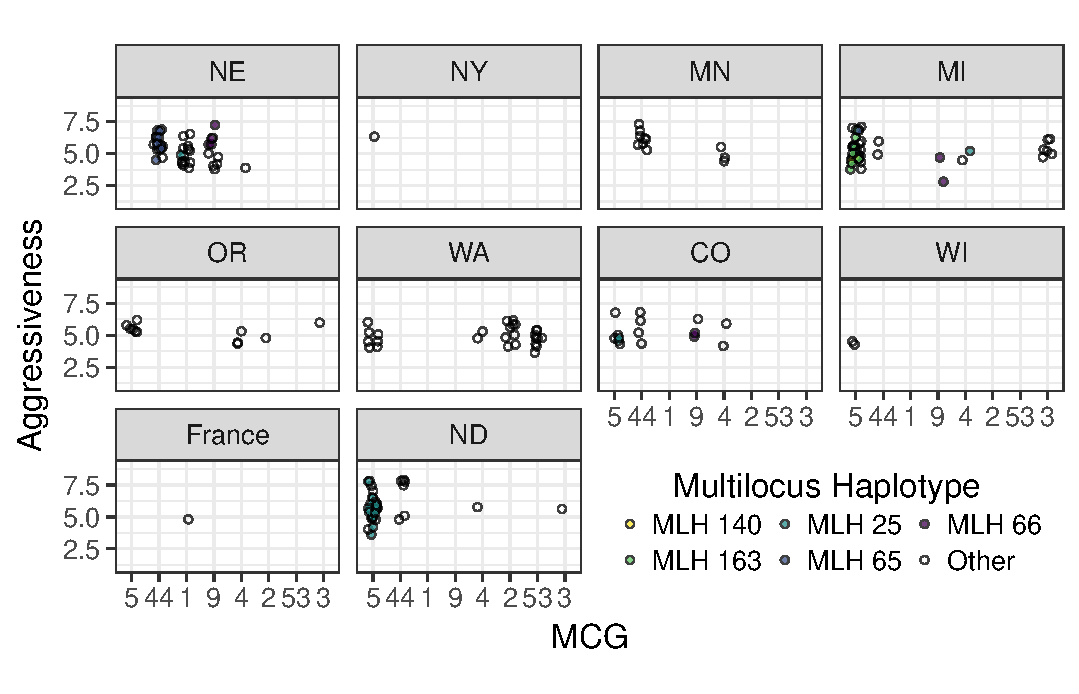
\includegraphics[width=1.00000\textwidth]{../../results/figures/publication/RMM-aggressiveness.pdf}
\caption{Strip plot of aggressiveness for the eight most abundant MCGs
partitioned by region. Filled circles indicate one of the five most
abundant MLHs and open circles indicate a MLH of lesser
abundance.}\label{mcg-mlh-region-aggressiveness}
\end{figure}

\begin{figure}
\centering
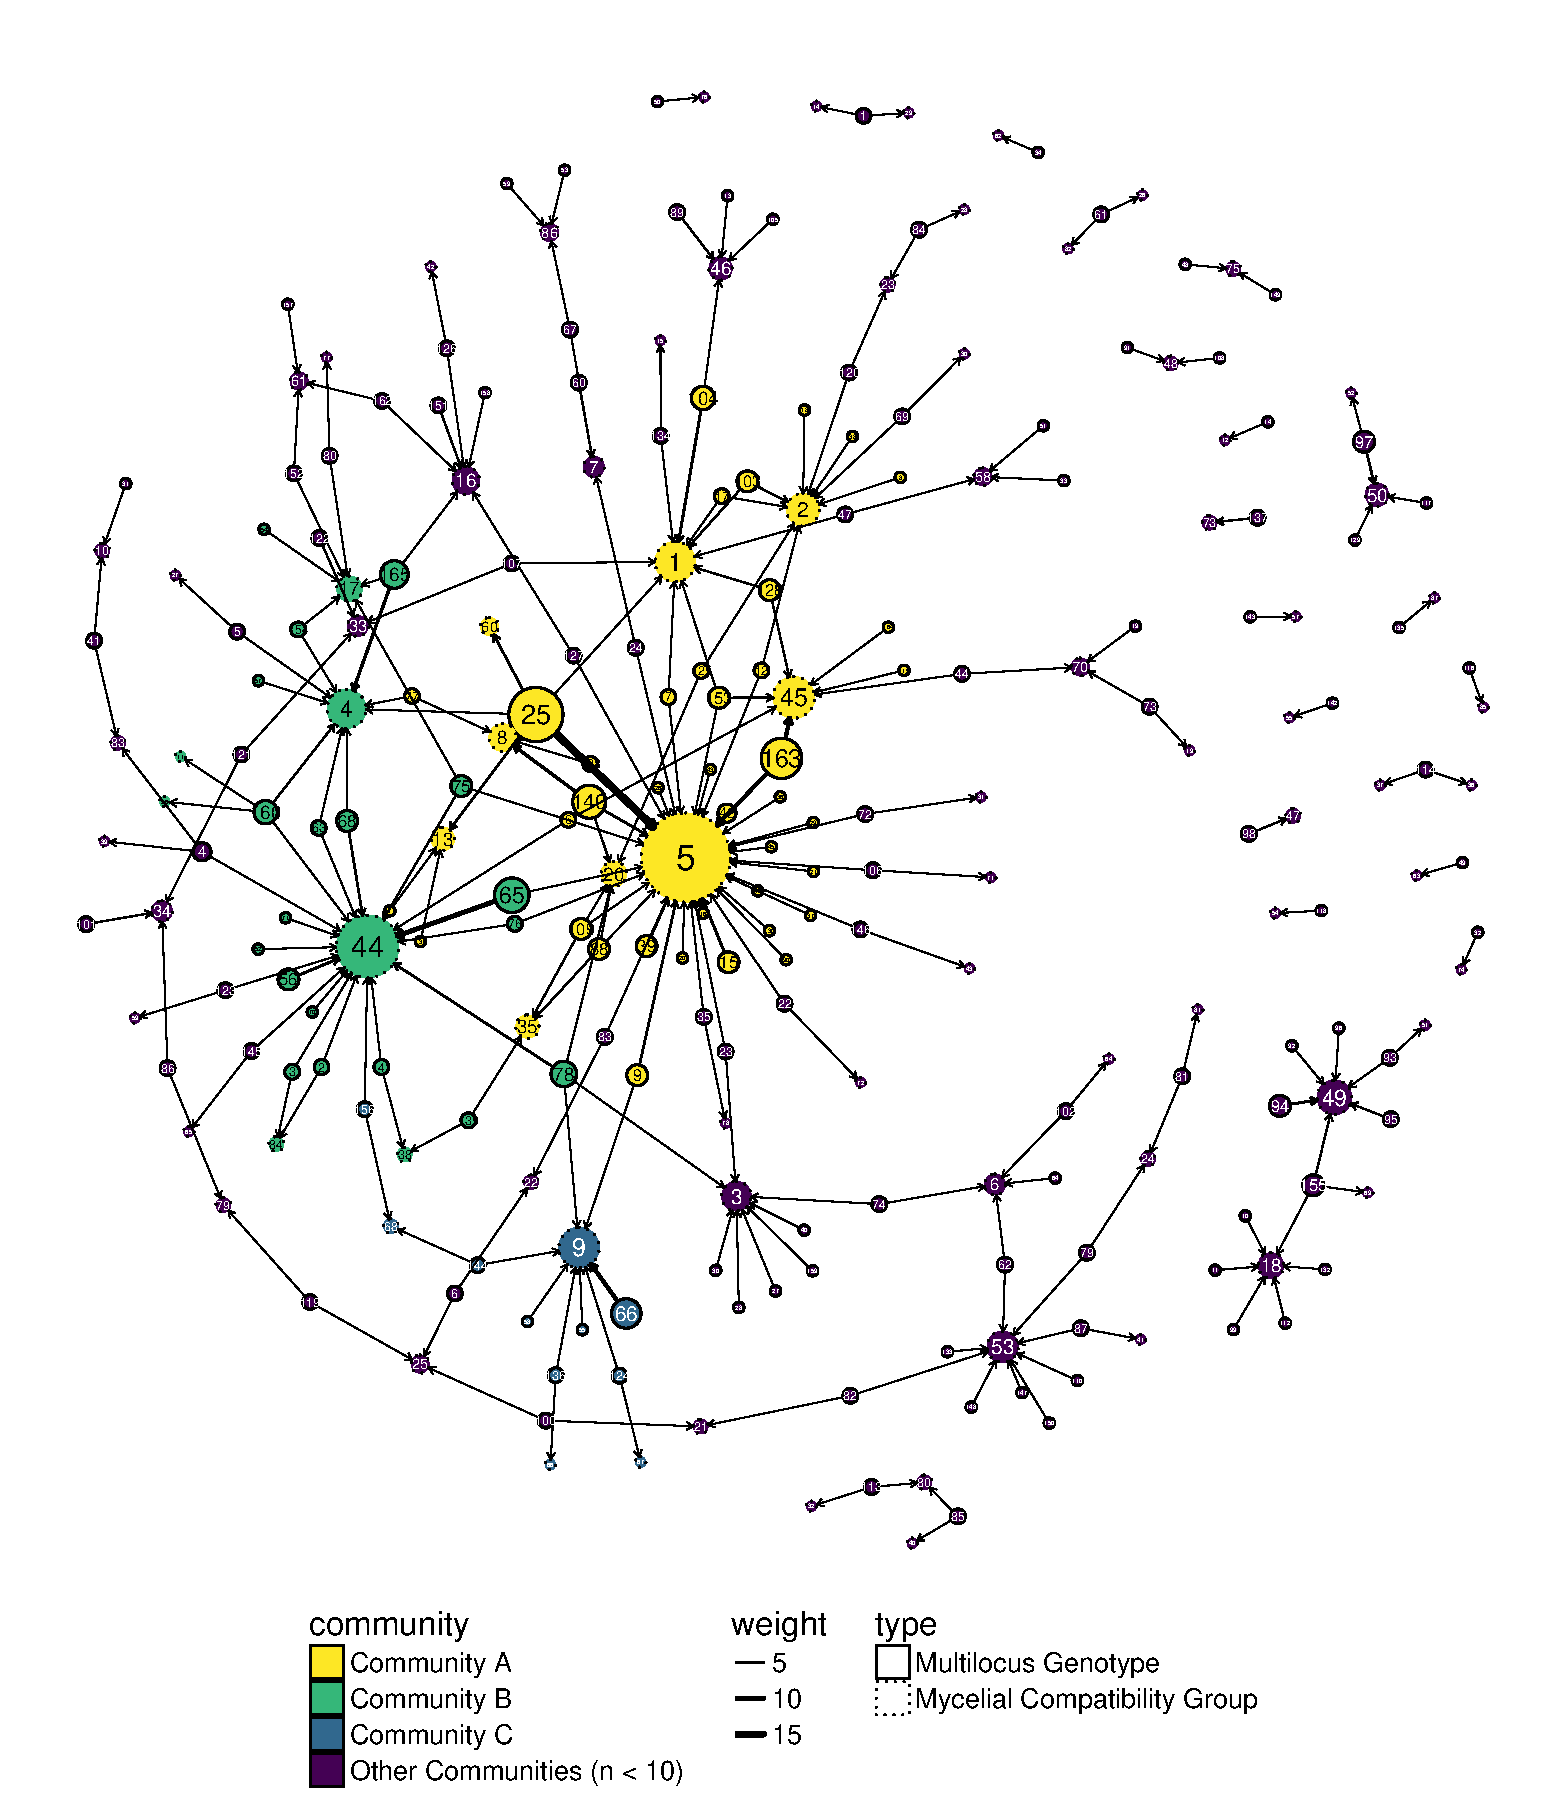
\includegraphics[width=1.00000\textwidth]{../../results/figures/publication/full-graph.pdf}
\caption{Graph showing complex associations between Mycelial
Compatibility Groups (MCG) (dotted nodes) and Multilocus Haplotypes
(MLH) (full nodes) where the number in each node represents the MLH/MCG
assignment. Node size reflect the number of samples represented by each
node (circle). Edges (arrows) point from MLH to MCG where the weight
(thickness) of the edge represents the number of samples shared. Node
color represents the community assignment based on the walktrap
algorithm with a maximum of four steps (Pons \& Latapy, 2006). An
interactive version of this network can be recreated using the code in
the ``Interactive visualizations'' section of the mlg-mcg.md file in the
supplementary information (Direct Link:
\url{https://github.com/everhartlab/sclerotinia-366/blob/master/results/mlg-mcg.md\#interactive-visualizations})
(Kamvar et al., 2017).}\label{fullgraph}
\end{figure}

\begin{figure}
\centering
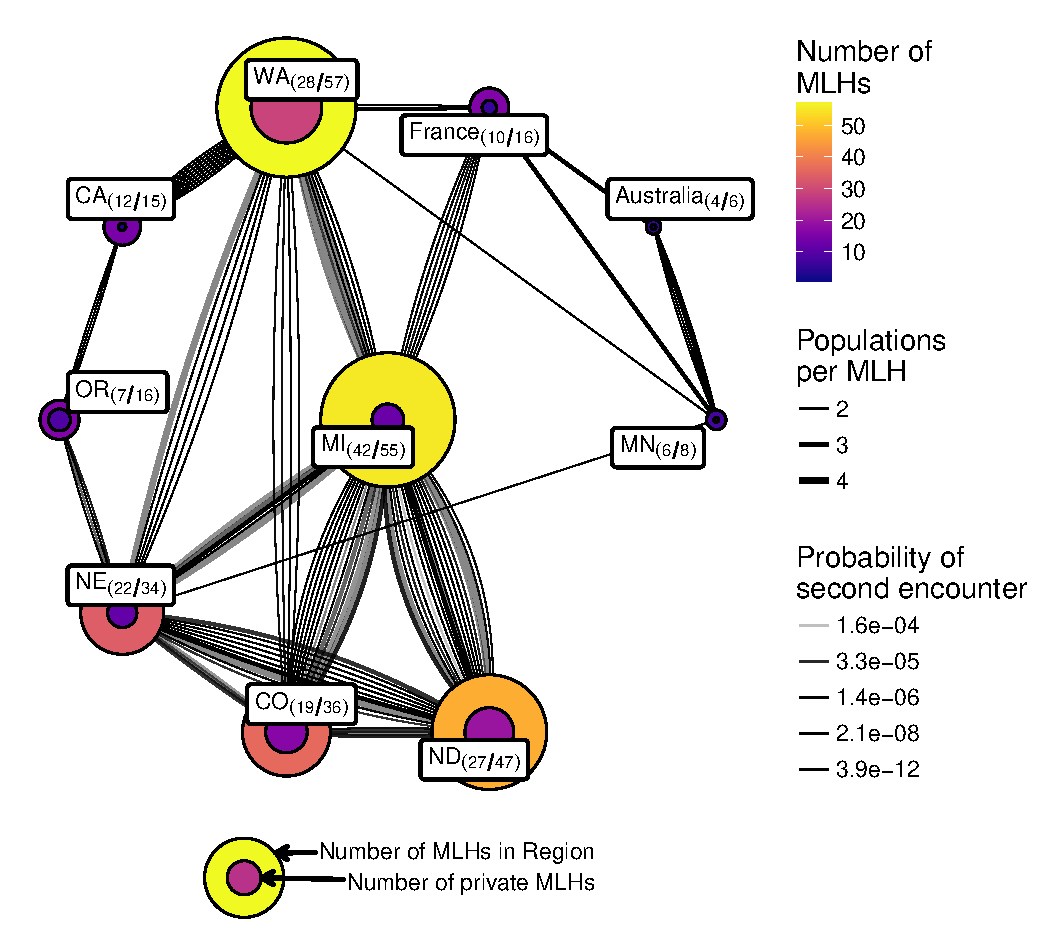
\includegraphics[width=1.00000\textwidth]{../../results/figures/publication/mlg-16.pdf}
\caption{Network of populations (nodes/circles) and their shared
multilocus haplotypes (MLH) (edges/lines) haplotyped over 16 loci. Each
node is labeled with \textbf{name (number of MLHs shared/number of MLHs
total).} The shade and area of the nodes are proportional to the number
of unique MLHs within the node and the inner nodes are proportional to
the number of private MLHs to the region (bottom legend). Each edge
represents a single MLH where its thickness represents the number of
populations that share the MLH and the shade represents the value of
\(P_{sex}\), or the probability of encountering that MLH from two
independent meiotic events.}\label{community-graph16}
\end{figure}

\begin{figure}
\centering
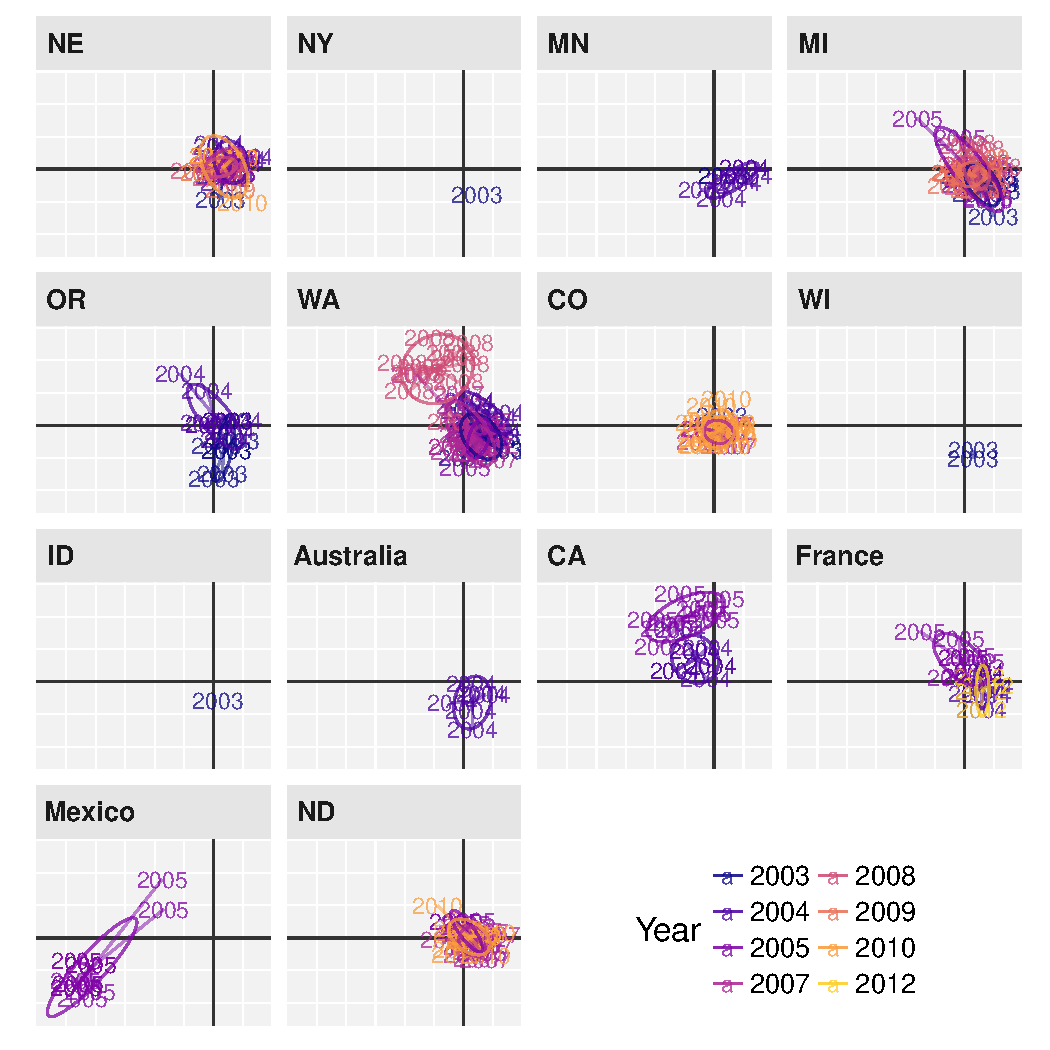
\includegraphics[width=1.00000\textwidth]{../../results/figures/publication/dapc_region_year.pdf}
\caption{Scatter plot of Discriminant Analysis of Principal Components
on Regions and Years showing temporal variation across all Regions.
Points (text labels) represent observed individuals connected to the
population centroids with ellipses representing a 66\% confidence
interval for a normal distribution. The center of each component is
represented as black grid lines.}\label{DAPC-RY-FULL}
\end{figure}

\newpage

\section*{References}\label{references}
\addcontentsline{toc}{section}{References}

\hypertarget{refs}{}
\hypertarget{ref-agapow2001indices}{}
Agapow, P., \& Burt, A. (2001). Indices of multilocus linkage
disequilibrium. \emph{Molecular Ecology Notes}, \emph{1}, 101--102.

\hypertarget{ref-aldrich-wolfe2015genetic}{}
Aldrich-Wolfe, L., Travers, S., \& Nelson, B. D. (2015). Genetic
variation of \emph{Sclerotinia sclerotiorum} from multiple crops in the
north central United States. \emph{PLOS ONE}, \emph{10}(9), e0139188.
\url{https://doi.org/10.1371/journal.pone.0139188}

\hypertarget{ref-arnaud2007standardizing}{}
Arnaud-Hanod, S., Duarte, C. M., Alberto, F., \& Serrão, E. A. (2007).
Standardizing methods to address clonality in population studies.
\emph{Molecular Ecology}, \emph{16}(24), 5115--5139.
\url{https://doi.org/10.1111/j.1365-294X.2007.03535.x}

\hypertarget{ref-atallah2004high}{}
Atallah, Z. K., Larget, B., Chen, X., \& Johnson, D. A. (2004). High
genetic diversity, phenotypic uniformity, and evidence of outcrossing in
\emph{Sclerotinia sclerotiorum} in the Columbia Basin of Washington
State. \emph{Phytopathology}, \emph{94}, 737--742.

\hypertarget{ref-attali2016ezknitr}{}
Attali, D. (2016). ezknitr: Avoid the typical working directory pain
when using ``knitr''. \emph{The Journal of Open Source Software},
\emph{1}(5), 75. \url{https://doi.org/10.21105/joss.00075}

\hypertarget{ref-attanayake2013sclerotinia}{}
Attanayake, R. N., Carter, P. A., Jiang, D., del Río-Mendoza, L., \&
Chen, W. (2013). \emph{Sclerotinia sclerotiorum} populations infecting
canola from China and the United States are genetically and
phenotypically distinct. \emph{Phytopathology}, \emph{103}(7), 750--761.
\url{https://doi.org/10.1094/phyto-07-12-0159-r}

\hypertarget{ref-attanayake2012genetic}{}
Attanayake, R., Porter, L., Johnson, D., \& Chen, W. (2012). Genetic and
phenotypic diversity and random association of DNA markers of isolates
of the fungal plant pathogen \emph{Sclerotinia sclerotiorum} from soil
on a fine geographic scale. \emph{Soil Biology and Biochemistry},
\emph{55}, 28--36. \url{https://doi.org/10.1016/j.soilbio.2012.06.002}

\hypertarget{ref-boettiger2017introduction}{}
Boettiger, C., \& Eddelbuettel, D. (2017). An introduction to rocker:
Docker containers for R. \emph{CoRR}, \emph{abs/1710.03675}. Retrieved
from \url{http://arxiv.org/abs/1710.03675}

\hypertarget{ref-boland1994index}{}
Boland, G., \& Hall, R. (1994). Index of plant hosts of
\emph{Sclerotinia sclerotiorum}. \emph{Canadian Journal of Plant
Pathology}, \emph{16}(2), 93--108.
\url{https://doi.org/10.1080/07060669409500766}

\hypertarget{ref-bolton2006sclerotinia}{}
Bolton, M. D., Thomma, B. P. H. J., \& Nelson, B. D. (2006).
\emph{Sclerotinia sclerotiorum} (Lib.) de Bary: Biology and molecular
traits of a cosmopolitan pathogen. \emph{Molecular Plant Pathology},
\emph{7}(1), 1--16.
\url{https://doi.org/10.1111/j.1364-3703.2005.00316.x}

\hypertarget{ref-botelho2013performance}{}
Botelho, L. d., Zancan, W. L. A., Cruz Machado, J. da, \& Barrocas, E.
N. (2013). Performance of common bean seeds infected by the fungus
\emph{Sclerotinia sclerotiorum}. \emph{Journal of Seed Science},
\emph{35}(2), 153--160.
\url{https://doi.org/10.1590/s2317-15372013000200003}

\hypertarget{ref-brown1980multilocus}{}
Brown, A. H. D., Feldman, M. W., \& Nevo, E. (1980). Multilocus
structure of natural populations of \emph{Hordeum Spontaneum}.
\emph{Genetics}, \emph{96}(2), 523--536. Retrieved from
\url{http://www.genetics.org/content/96/2/523}

\hypertarget{ref-bruvo2004simple}{}
Bruvo, R., Michiels, N. K., D'Souza, T. G., \& Schulenburg, H. (2004). A
simple method for the calculation of microsatellite genotype distances
irrespective of ploidy level. \emph{Molecular Ecology}, \emph{13}(7),
2101--2106.

\hypertarget{ref-carbone2001multilocus}{}
Carbone, I., \& Kohn, L. M. (2001). Multilocus nested haplotype networks
extended with DNA fingerprints show common origin and fine-scale,
ongoing genetic divergence in a wild microbial metapopulation.
\emph{Molecular Ecology}, \emph{10}(10), 2409--2422.
\url{https://doi.org/10.1046/j.0962-1083.2001.01380.x}

\hypertarget{ref-carbone1999patterns}{}
Carbone, I., Anderson, J. B., \& Kohn, L. M. (1999). Patterns of descent
in clonal lineages and their multilocus fingerprints are resolved with
combined gene genealogies. \emph{Evolution}, \emph{53}(1), 11--21.
\url{https://doi.org/10.1111/j.1558-5646.1999.tb05329.x}

\hypertarget{ref-csardi2006igraph}{}
Csardi, G., \& Nepusz, T. (2006). The igraph software package for
complex network research. \emph{InterJournal}, \emph{Complex Systems},
1695. Retrieved from \url{http://igraph.org}

\hypertarget{ref-cubeta1997clonality}{}
Cubeta, M. A., Cody, B. R., Kohli, Y., \& Kohn, L. M. (1997). Clonality
in \emph{Sclerotinia sclerotiorum} on infected cabbage in eastern North
Carolina. \emph{Phytopathology}, \emph{87}, 1000--1004.

\hypertarget{ref-cubeta2001mycelial}{}
Cubeta, M., Sermons, D., \& Cody, B. (2001). Mycelial interactions of
\emph{Sclerotinia minor}. \emph{Phytopathology}, \emph{91}(6S), S19.
\url{https://doi.org/10.1094/phyto.2001.91.6.s1}

\hypertarget{ref-davey2011genome}{}
Davey, J. W., Hohenlohe, P. A., Etter, P. D., Boone, J. Q., Catchen, J.
M., \& Blaxter, M. L. (2011). Genome-wide genetic marker discovery and
genotyping using next-generation sequencing. \emph{Nature Reviews
Genetics}, \emph{12}(7), 499--510. \url{https://doi.org/10.1038/nrg3012}

\hypertarget{ref-derbyshire2017complete}{}
Derbyshire, M., Denton-Giles, M., Hegedus, D., Seifbarghy, S., Rollins,
J., van Kan, J., Seidl, M. F., Faino, L., Mbengue, M., Navaud, O.,
Raffaele, S., Hammond-Kosack, K., Heard, S., \& Oliver, R. (2017). The
complete genome sequence of the phytopathogenic fungus \emph{Sclerotinia
sclerotiorum} reveals insights into the genome architecture of broad
host range pathogens. \emph{Genome Biology and Evolution}, \emph{9}(3),
593--618. \url{https://doi.org/10.1093/gbe/evx030}

\hypertarget{ref-ekins2011population}{}
Ekins, M. G., Hayden, H. L., Aitken, E. A. B., \& Goulter, K. C. (2011).
Population structure of \emph{Sclerotinia sclerotiorum} on sunflower in
Australia. \emph{Australasian Plant Pathology}, \emph{40}, 99--108.

\hypertarget{ref-excoffier1992analysis}{}
Excoffier, L., Smouse, P. E., \& Quattro, J. M. (1992). Analysis of
molecular variance inferred from metric distances among DNA haplotypes:
Application to human mitochondrial DNA restriction data.
\emph{Genetics}, \emph{131}(2), 479--91.

\hypertarget{ref-ford1995heterokaryon}{}
Ford, E., Miller, R., Gray, H., \& Sherwood, J. (1995). Heterokaryon
formation and vegetative compatibility in \emph{Sclerotinia
sclerotiorum}. \emph{Mycological Research}, \emph{99}(2), 241--247.

\hypertarget{ref-grover2012targeted}{}
Grover, C. E., Salmon, A., \& Wendel, J. F. (2012). Targeted sequence
capture as a powerful tool for evolutionary analysis. \emph{American
Journal of Botany}, \emph{99}(2), 312--319.
\url{https://doi.org/10.3732/ajb.1100323}

\hypertarget{ref-grunwald2003analysis}{}
Grünwald, N. J., Goodwin, S. B., Milgroom, M. G., \& Fry, W. E. (2003).
Analysis of genotypic diversity data for populations of microorganisms.
\emph{Phytopathology}, \emph{93}(6), 738--746.
\url{https://doi.org/10.1094/phyto.2003.93.6.738}

\hypertarget{ref-hall2010evolution}{}
Hall, C., Welch, J., Kowbel, D. J., \& Glass, N. L. (2010). Evolution
and diversity of a fungal self/nonself recognition locus. \emph{PLoS
ONE}, \emph{5}(11), e14055.
\url{https://doi.org/10.1371/journal.pone.0014055}

\hypertarget{ref-heck1975explicit}{}
Heck, K. L., van Belle, G., \& Simberloff, D. (1975). Explicit
calculation of the rarefaction diversity measurement and the
determination of sufficient sample size. \emph{Ecology}, \emph{56}(6),
1459--1461. \url{https://doi.org/10.2307/1934716}

\hypertarget{ref-purrr}{}
Henry, L., \& Wickham, H. (2017). \emph{purrr: Functional programming
tools}. Retrieved from \url{https://CRAN.R-project.org/package=purrr}

\hypertarget{ref-hurlbert1971nonconcept}{}
Hurlbert, S. H. (1971). The nonconcept of species diversity: A critique
and alternative parameters. \emph{Ecology}, \emph{52}(4), 577--586.
\url{https://doi.org/10.2307/1934145}

\hypertarget{ref-jo2008reassessment}{}
Jo, Y.-K., Chang, S. W., Rees, J., \& Jung, G. (2008). Reassessment of
vegetative compatibility of \emph{Sclerotinia homoeocarpa} using
nitrate-nonutilizing mutants. \emph{Phytopathology}, \emph{98}(1),
108--114. \url{https://doi.org/10.1094/phyto-98-1-0108}

\hypertarget{ref-jombart2008adegenet}{}
Jombart, T. (2008). adegenet: A R package for the multivariate analysis
of genetic markers. \emph{Bioinformatics}, \emph{24}(11), 1403--1405.
\url{https://doi.org/10.1093/bioinformatics/btn129}

\hypertarget{ref-jombart2010discriminant}{}
Jombart, T., Devillard, S., \& Balloux, F. (2010). Discriminant analysis
of principal components: A new method for the analysis of genetically
structured populations. \emph{BMC Genetics}, \emph{11:94}.
\url{https://doi.org/10.1186/1471--2156--11--94}

\hypertarget{ref-kamvar2017data}{}
Kamvar, Z. N., Amaradasa, B. S., Jhala, R., McCoy, S., Steadman, J. R.,
\& Everhart, S. E. (2017, November). Data and analysis for population
structure and phenotypic variation of \emph{Sclerotinia sclerotiorum}
from dry bean (\emph{Phaseolus vulgaris}) in the United States. Open
Science Framework. \url{https://doi.org/10.17605/OSF.IO/K8WTM}

\hypertarget{ref-kamvar2015novel}{}
Kamvar, Z. N., Brooks, J. C., \& Grünwald, N. J. (2015). Novel R tools
for analysis of genome-wide population genetic data with emphasis on
clonality. \emph{Frontiers in Genetics}, \emph{6}, 208.
\url{https://doi.org/10.3389/fgene.2015.00208}

\hypertarget{ref-kamvar2014poppr}{}
Kamvar, Z. N., Tabima, J. F., \& Grünwald, N. J. (2014). Poppr: An R
package for genetic analysis of populations with clonal, partially
clonal, and/or sexual reproduction. \emph{PeerJ}, \emph{2}, e281.
\url{https://doi.org/10.7717/peerj.281}

\hypertarget{ref-knodel2012dry}{}
Knodel, J., Beauzay, P., Franzen, D., Kandel, H., Markell, S., Osorno,
J., Pasche, J., \& Zollinger, R. (2012). 2012 dry bean grower survey of
production, pest problems and pesticide use in Minnesota and North
Dakota. \emph{North Dakota State University Extension}, \emph{E1640}.

\hypertarget{ref-knodel2015dry}{}
Knodel, J., Beauzay, P., Franzen, D., Kandel, H., Markell, S., Osorno,
J., Pasche, J., \& Zollinger, R. (2015). 2015 dry bean grower survey of
production, pest problems and pesticide use in Minnesota and North
Dakota. \emph{North Dakota State University Extension}, \emph{E1802}.

\hypertarget{ref-knodel2016dry}{}
Knodel, J., Beauzay, P., Franzen, D., Kandel, H., Markell, S., Osorno,
J., Pasche, J., \& Zollinger, R. (2016). 2016 dry bean grower survey of
production, pest problems and pesticide use in Minnesota and North
Dakota. \emph{North Dakota State University Extension}, \emph{E1841}.

\hypertarget{ref-kohli1998random}{}
Kohli, Y., \& Kohn, L. M. (1998). Random association among alleles in
clonal populations of \emph{Sclerotinia sclerotiorum}. \emph{Fungal
Genetics and Biology}, \emph{23}, 139--149.

\hypertarget{ref-kohli1995clonal}{}
Kohli, Y., Brunner, L. J., Yoell, H., Milgroom, M. G., Anderson, J. B.,
Morrall, R. A. A., \& Kohn, L. M. (1995). Clonal dispersal and spatial
mixing in populations of the plant pathogenic fungus, \emph{Sclerotinia
sclerotiorum}. \emph{Molecular Ecology}, \emph{4}, 69--77.

\hypertarget{ref-kohn1995clonal}{}
Kohn, L. M. (1995). The clonal dynamic in wild and agricultural
plant-pathogen populations. \emph{Canadian Journal of Botany},
\emph{73}(S1), 1231--1240. \url{https://doi.org/10.1139/b95-383}

\hypertarget{ref-kohn1990mycelial}{}
Kohn, L. M., Carbone, I., \& Anderson, J. B. (1990). Mycelial
interactions in \emph{Sclerotinia sclerotiorum}. \emph{Experimental
Mycology}, \emph{14}, 255--267.

\hypertarget{ref-legendre1999distance}{}
Legendre, P., \& Anderson, M. J. (1999). Distance-based redundancy
analysis: Testing multispecies responses in multifactorial ecological
experiments. \emph{Ecological Monographs}, \emph{69}, 1--24.

\hypertarget{ref-lehner2017sclerotinia}{}
Lehner, M. S., \& Mizubuti, E. S. G. (2017). Are \emph{Sclerotinia
sclerotiorum} populations from the tropics more variable than those from
subtropical and temperate zones? \emph{Tropical Plant Pathology},
\emph{42}(2), 61--69. \url{https://doi.org/10.1007/s40858-016-0125-1}

\hypertarget{ref-lehner2015genetic}{}
Lehner, M. S., Júnior, T. J. P., Júnior, B. T. H., Teixeira, H., Vieira,
R. F., Carneiro, J. E. S., \& Mizubuti, E. S. G. (2015). Low genetic
variability in \emph{Sclerotinia sclerotiorum} populations from common
bean fields in Minas Gerais State, Brazil, at regional, local and
micro-scales. \emph{Plant Pathology}, \emph{64}(4), 921--931.
\url{https://doi.org/10.1111/ppa.12322}

\hypertarget{ref-lehner2017independently}{}
Lehner, M. S., Paula Júnior, T. J. de, Del Ponte, E. M., Mizubuti, E.
S., \& Pethybridge, S. J. (2017). Independently founded populations of
\emph{Sclerotinia sclerotiorum} from a tropical and a temperate region
have similar genetic structure. \emph{PloS One}, \emph{12}(3), e0173915.
\url{https://doi.org/10.1371/journal.pone.0173915}

\hypertarget{ref-leslie1993fungal}{}
Leslie, J. (1993). Fungal vegetative compatibility. \emph{Annual Review
of Phytopathology}, \emph{31}, 127--150. Review.
\url{https://doi.org/10.1146/annurev.py.31.090193.001015}

\hypertarget{ref-mccoy2009use}{}
McCoy, S., \& Steadman, J. R. (2009). Use of multi-site screening to
identify partial resistance to white mold in common bean in 2008.
\emph{Bean Improvement Cooperative Annual Report}, \emph{52}, 86--87.
Retrieved from
\url{https://naldc.nal.usda.gov/naldc/catalog.xhtml?id=IND44207142}

\hypertarget{ref-mcdonald2002pathogen}{}
McDonald, B. A., \& Linde, C. (2002). Pathogen population genetics,
evolutionary potential, and durable resistance. \emph{Annual Review of
Phytopathology}, \emph{40}(1), 349--379.
\url{https://doi.org/10.1146/annurev.phyto.40.120501.101443}

\hypertarget{ref-mendiburu2015agricolae}{}
Mendiburu, F. D., \& Simon, R. (2015). Agricolae - ten years of an open
source statistical tool for experiments in breeding, agriculture and
biology. \emph{PeerJ PrePrints}, \emph{3}, e1404v1.
\url{https://doi.org/10.7287/peerj.preprints.1404v1}

\hypertarget{ref-micali2003independence}{}
Micali, C. O., \& Smith, M. L. (2003). On the independence of barrage
formation and heterokaryon incompatibility in \emph{Neurospora crassa}.
\emph{Fungal Genetics and Biology}, \emph{38}(2), 209--219.
\url{https://doi.org/10.1016/s1087-1845(02)00533-9}

\hypertarget{ref-milgroom1996recombination}{}
Milgroom, M. G. (1996). Recombination and the multilocus structure of
fungal populations. \emph{Annual Review of Phytopathology},
\emph{34}(1), 457--477.

\hypertarget{ref-nei1978estimation}{}
Nei, M. (1978). Estimation of average heterozygosity and genetic
distance from a small number of individuals. \emph{Genetics}, \emph{89},
583--590.

\hypertarget{ref-vegan}{}
Oksanen, J., Blanchet, F. G., Friendly, M., Kindt, R., Legendre, P.,
McGlinn, D., Minchin, P. R., O'Hara, R. B., Simpson, G. L., Solymos, P.,
Stevens, M. H. H., Szoecs, E., \& Wagner, H. (2017). \emph{Vegan:
Community ecology package}. Retrieved from
\url{https://CRAN.R-project.org/package=vegan}

\hypertarget{ref-otto2007identification}{}
Otto-Hanson, L., \& Steadman, J. R. (2007). Identification of partial
resistance to \emph{Sclerotinia sclerotiorum} in common bean at multiple
locations in 2006. \emph{Bean Improvement Cooperative Annual Report},
\emph{50}, 133--134. Retrieved from
\url{https://naldc.nal.usda.gov/naldc/catalog.xhtml?id=IND43940892}

\hypertarget{ref-otto2008identification}{}
Otto-Hanson, L., \& Steadman, J. R. (2008). Identification of partial
resistance to \emph{Sclerotinia sclerotiorum} in common bean at multiple
locations in 2007. \emph{Bean Improvement Cooperative Annual Report},
\emph{51}, 214--215. Retrieved from
\url{https://naldc.nal.usda.gov/naldc/catalog.xhtml?id=IND44063230}

\hypertarget{ref-otto-hanson2011variation}{}
Otto-Hanson, L., Steadman, J. R., Higgins, R., \& Eskridge, K. M.
(2011). Variation in \emph{Sclerotinia sclerotiorum} bean isolates from
multisite resistance screening locations. \emph{Plant Disease},
\emph{95}(11), 1370--1377. \url{https://doi.org/10.1094/pdis-11-10-0865}

\hypertarget{ref-papaioannou2014barrage}{}
Papaioannou, I. A., \& Typas, M. A. (2014). Barrage formation is
independent from heterokaryon incompatibility in \emph{Verticillium
dahliae}. \emph{European Journal of Plant Pathology}, \emph{141}(1),
71--82. \url{https://doi.org/10.1007/s10658-014-0525-3}

\hypertarget{ref-parks1993study}{}
Parks, J. C., \& Werth, C. R. (1993). A study of spatial features of
clones in a population of bracken fern, \emph{Pteridium aquilinum}
(Dennstaedtiaceae). \emph{American Journal of Botany}, \emph{80}(5),
537. \url{https://doi.org/10.2307/2445369}

\hypertarget{ref-ggraph}{}
Pedersen, T. L. (2017). \emph{ggraph: An implementation of grammar of
graphics for graphs and networks}. Retrieved from
\url{https://CRAN.R-project.org/package=ggraph}

\hypertarget{ref-petzoldt1996straw}{}
Petzoldt, R., \& Dickson, M. H. (1996). Straw test for resistance to
white mold in beans. \emph{Bean Improvement Cooperative Annual Report},
\emph{39}, 142--143. Retrieved from
\url{https://naldc.nal.usda.gov/naldc/catalog.xhtml?id=IND20562675}

\hypertarget{ref-pielou1975ecological}{}
Pielou, E. (1975). \emph{Ecological Diversity}. New York: Wiley \& Sons.

\hypertarget{ref-pons2006computing}{}
Pons, P., \& Latapy, M. (2006). Computing communities in large networks
using random walks. \emph{Journal of Graph Algorithms and Applications},
\emph{10}(2), 191--218. \url{https://doi.org/10.7155/jgaa.00124}

\hypertarget{ref-prugnolle2010apparent}{}
Prugnolle, F., \& de Meeûs, T. (2010). Apparent high recombination rates
in clonal parasitic organisms due to inappropriate sampling design.
\emph{Heredity}, \emph{104}(2), 135--140.
\url{https://doi.org/10.1038/hdy.2009.128}

\hypertarget{ref-R}{}
R Core Team. (2017). \emph{R: A language and environment for statistical
computing}. Vienna, Austria: R Foundation for Statistical Computing.
Retrieved from \url{https://www.R-project.org/}

\hypertarget{ref-ramasubramaniam2008estimates}{}
Ramasubramaniam, H., del Río Mendoza, L. E., \& Bradley, C. A. (2008).
Estimates of yield and economic losses associated with white mold of
rain-fed dry bean in North Dakota. \emph{Agronomy Journal},
\emph{100}(2), 315. \url{https://doi.org/10.2134/agronj2007.0127}

\hypertarget{ref-sambrook1989molecular}{}
Sambrook, J., Fritsch, E. F., Maniatis, T., \& others. (1989).
\emph{Molecular Cloning: A Laboratory Manual.} Cold spring harbor
laboratory press.

\hypertarget{ref-saupe2000molecular}{}
Saupe, S. J. (2000). Molecular genetics of heterokaryon incompatibility
in filamentous ascomycetes. \emph{Microbiology and Molecular Biology
Reviews}, \emph{64}(3), 489--502.
\url{https://doi.org/10.1128/mmbr.64.3.489-502.2000}

\hypertarget{ref-schafer2006optimized}{}
Schafer, M. R., \& Kohn, L. M. (2006). An optimized method for mycelial
compatibility testing in \emph{Sclerotinia sclerotiorum}.
\emph{Mycologia}, \emph{98}(4), 593--597.
\url{https://doi.org/10.1080/15572536.2006.11832662}

\hypertarget{ref-sexton2004microsatellite}{}
Sexton, A. C., \& Howlett, B. J. (2004). Microsatellite markers reveal
genetic differentiation among populations of \emph{Sclerotinia
sclerotiorum} from Australian canola fields. \emph{Current Genetics},
\emph{46}(6), 357--365. \url{https://doi.org/10.1007/s00294-004-0543-3}

\hypertarget{ref-sexton2006population}{}
Sexton, A. C., Whitten, A. R., \& Howlett, B. J. (2006). Population
structure of \emph{Sclerotinia sclerotiorum} in an Australian canola
field at flowering and stem-infection stages of the disease cycle.
\emph{Genome}, \emph{49}(11), 1408--1415.
\url{https://doi.org/10.1139/g06-101}

\hypertarget{ref-shannon2001mathematical}{}
Shannon, C. E. (1948). A mathematical theory of communication. \emph{ACM
SIGMOBILE Mobile Computing and Communications Review}, \emph{5}(1),
3--55.

\hypertarget{ref-simpson1949measurement}{}
Simpson, E. H. (1949). Measurement of diversity. \emph{Nature},
\emph{163}(4148), 688--688. \url{https://doi.org/10.1038/163688a0}

\hypertarget{ref-sirjusingh2001characterisation}{}
Sirjusingh, C., \& Kohn, L. M. (2001). Characterisation of
microsatellites in the fungal plant pathogen, \emph{Sclerotinia
sclerotiorum}. \emph{Molecular Ecology Notes}, \emph{1}(4), 267--269.
\url{https://doi.org/10.1046/j.1471-8278.2001.00102.x}

\hypertarget{ref-smith1993how}{}
Smith, J. M., Smith, N. H., O'Rourke, M., \& Spratt, B. G. (1993). How
clonal are bacteria? \emph{Proceedings of the National Academy of
Sciences}, \emph{90}(10), 4384--4388.
\url{https://doi.org/10.1073/pnas.90.10.4384}

\hypertarget{ref-steadman1983white}{}
Steadman, J. R. (1983). White mold - a serious yield-limiting disease of
bean. \emph{Plant Disease}, \emph{67}, 346--350.

\hypertarget{ref-steadman2003identification}{}
Steadman, J. R., Eskridge, K., \& Powers, K. (2003). Identification of
partial resistance to \emph{Sclerotinia sclerotiorum} in common bean at
multiple locations. \emph{Bean Improvement Cooperative Annual Report},
\emph{46}, 225--226. Retrieved from
\url{https://naldc.nal.usda.gov/naldc/catalog.xhtml?id=IND43757287}

\hypertarget{ref-steadman2006identification}{}
Steadman, J. R., Otto-Hanson, L., \& Breathnach, J. (2006).
Identification of partial resistance to \emph{Sclerotinia sclerotiorum}
in common bean at multiple locations in 2005. \emph{Bean Improvement
Cooperative Annual Report}, \emph{49}, 223--224. Retrieved from
\url{https://naldc.nal.usda.gov/naldc/catalog.xhtml?id=IND43805570}

\hypertarget{ref-steadman2004identification}{}
Steadman, J. R., Otto-Hanson, L., \& Powers, K. (2004). Identification
of partial resistance to \emph{Sclerotinia sclerotiorum} in common bean
at multiple locations. \emph{Bean Improvement Cooperative Annual
Report}, \emph{47}, 281--282. Retrieved from
\url{https://naldc.nal.usda.gov/naldc/catalog.xhtml?id=IND43758354}

\hypertarget{ref-steadman2005identification}{}
Steadman, J. R., Otto-Hanson, L., \& Powers, K. (2005). Identification
of partial resistance to \emph{Sclerotinia sclerotiorum} in common bean
at multiple locations in 2004. \emph{Bean Improvement Cooperative Annual
Report}, \emph{48}, 124--125. Retrieved from
\url{https://naldc.nal.usda.gov/naldc/catalog.xhtml?id=IND43759243}

\hypertarget{ref-stoddart1988genotypic}{}
Stoddart, J. A., \& Taylor, J. F. (1988). Genotypic diversity:
Estimation and prediction in samples. \emph{Genetics}, \emph{118}(4),
705--11.

\hypertarget{ref-strausbaugh2003management}{}
Strausbaugh, C., \& Forster, R. (2003). Management of white mold of
beans. \emph{Pacific Northwest Extension}, \emph{PNW568}. Retrieved from
\url{http://http://www.extension.uidaho.edu/publishing/pdf/PNW/PNW0568.pdf}

\hypertarget{ref-strom2016genomes}{}
Strom, N. B., \& Bushley, K. E. (2016). Two genomes are better than one:
History, genetics, and biotechnological applications of fungal
heterokaryons. \emph{Fungal Biology and Biotechnology}, \emph{3}(1).
\url{https://doi.org/10.1186/s40694-016-0022-x}

\hypertarget{ref-teran2006modified}{}
Teran, H., Lema, M., Schwartz, H. F., Duncan, R., Gilbeitson, R., \&
Singh, S. P. (2006). Modified Petzoldt and Dickson scale for white mold
rating of common bean. \emph{Bean Improvement Cooperative Annual
Report}, \emph{49}, 115--116. Retrieved from
\url{https://naldc.nal.usda.gov/naldc/catalog.xhtml?id=IND43805401}

\hypertarget{ref-tu1982tolerance}{}
Tu, J. C., \& Beversdorf, W. D. (1982). Tolerance to white mold
(\emph{Sclerotinia sclerotiorum} (Lib.) De Bary) in Ex Rico 23, a
cultivar of white bean (\emph{Phaseolus vulgaris} L.). \emph{Canadian
Journal of Plant Science}, \emph{62}(1), 65--69.
\url{https://doi.org/10.4141/cjps82-010}

\hypertarget{ref-ggplot2}{}
Wickham, H. (2009). \emph{ggplot2: Elegant graphics for data analysis}.
Springer-Verlag New York. Retrieved from \url{http://ggplot2.org}

\hypertarget{ref-dplyr}{}
Wickham, H., Francois, R., Henry, L., \& Müller, K. (2017). \emph{dplyr:
A grammar of data manipulation}. Retrieved from
\url{https://CRAN.R-project.org/package=dplyr}

\hypertarget{ref-xie2017knitr}{}
Xie, Y. (2017). \emph{knitr: A general-purpose package for dynamic
report generation in R}. Retrieved from \url{https://yihui.name/knitr/}



\end{document}
